\documentclass[twocolumn]{svjour3}          % twocolumn
%
\smartqed  % flush right qed marks, e.g. at end of proof
%
\usepackage{graphicx}
\usepackage{enumerate}
\usepackage{latexsym}
\usepackage{amsfonts}
\usepackage{amsmath}
\usepackage{amssymb}
\usepackage[bigsqcap]{stmaryrd}
\usepackage{color}
\usepackage{colortbl}
\usepackage{epsfig}
\usepackage{xspace}
\usepackage{graphicx}
\usepackage{esvect} % for arrows
\usepackage{subfigure}
\usepackage{balance}
\usepackage{cite}
\usepackage[english]{babel}

%%%%%%%%%%%%%%%%%%%%%%%%%%%%%%%%%%%%%
%% DO NOT DELETE!!
%%%%%%%%%%%%%%%%%%%%%%%%%%%%%%%%%%%%%
%\usepackage{tikz}
%\usetikzlibrary{trees}

\usepackage{multirow}
\usepackage{url}


%%%%%%%%%%%%%%%%%%%%%%%%%%%%%%%%%%%%%%%%%%%%%%%%%%%%%%%%%%
\newcommand{\imp}{\vdash_{\cal I}}


%%%%%%%%%%%%%%%%%%%%%%%%%%%%%%%%%%%%%%%%%%
% Enumerate and Itemize modifications
%\usepackage{enumitem}
%\setlist{topsep=0pt,noitemsep} \setitemize[1]{label=$\circ$}
%%%%%%%%%%%%%%%%%%%%%%%%%%%%%%%%%%%%%%%%%%%

\sloppy
\newcommand{\rtable}[1]{\ensuremath{\mathsf{#1}}}
\newcommand{\ratt}[1]{\ensuremath{\mathit{#1}}}
\newcommand{\at}[1]{\protect\ensuremath{\mathsf{#1}}\xspace}
\newcommand{\myhrule}{\rule[.5pt]{\hsize}{.5pt}}
\newcommand{\oneurl}[1]{\texttt{#1}}
\newcommand{\eat}[1]{}
\newcommand{\stab}{\rule{0pt}{8pt}\\[-1.6ex]}
\newcommand{\sttab}{\rule{0pt}{8pt}\\[-2ex]}
%\newcommand{\sstab}{\rule{0pt}{8pt}\\[-2.4ex]}
\newcommand{\tabstrut}{\rule{0pt}{4pt}\vspace{-0.07in}}
\newcommand{\vs}{\vspace{1ex}}
\newcommand{\exa}[2]{{\tt\begin{tabbing}\hspace{#1}\=\+\kill #2\end{tabbing}}}
\newcommand{\ra}{\rightarrow}
\newcommand{\la}{\leftarrow}
\newcommand{\bi}{\begin{itemize}}
\newcommand{\ei}{\end{itemize}}
\newenvironment{tbi}{\begin{itemize}
        \setlength{\topsep}{1.5ex}\setlength{\itemsep}{0ex}\vspace{-0.5ex}}
        {\end{itemize}\vspace{-0.5ex}}
\newenvironment{tbe}{\begin{enumerate}
        \setlength{\topsep}{0ex}\setlength{\itemsep}{-0.7ex}\vspace{-1ex}}
        {\end{itemize}\vspace{-1ex}}

\newcommand{\mat}[2]{{\begin{tabbing}\hspace{#1}\=\+\kill #2\end{tabbing}}}
\newcommand{\m}{\hspace{0.05in}}
\newcommand{\ls}{\hspace{0.1in}}
\newcommand{\be}{\begin{enumerate}}
\newcommand{\ee}{\end{enumerate}}
\newcommand{\beqn}{\begin{eqnarray*}}
\newcommand{\eeqn}{\end{eqnarray*}}
\newcommand{\card}[1]{\mid\! #1\!\mid}
\newcommand{\fth}{\hfill $\Box$}
\newcommand{\AND}{\displaystyle{\bigwedge_{i=1}^{n}}}
%\newcommand{\U}[1]{\displaystyle{\bigcup_{#1}}}
\newcommand{\Sm}[1]{\displaystyle{\sum_{#1}}}
\newcommand{\stitle}[1]{\vspace{1ex}\noindent{\bf #1}}
\newcommand{\etitle}[1]{\vspace{0.5ex}\noindent{\em \underline{#1}}}
\renewcommand{\t}{\tau}
\newcommand{\Inh}[1]{\$#1}
\renewcommand{\r}[1]{{\it rule}(#1)}
\newcommand{\pa}{\parallel}
\newcommand{\LHS}{\kw{{\small LHS}}}
\newcommand{\RHS}{\kw{RHS}}
\newcommand{\len}{\kw{len}}
\newcommand{\kop}{\kw{op}}
%\newcommand{\st}{\emph{s.t.}\xspace}
\newcommand{\ie}{\emph{i.e.,}\xspace}
\newcommand{\eg}{\emph{e.g.,}\xspace}
\newcommand{\wrt}{\emph{w.r.t.}\xspace}
\newcommand{\aka}{\emph{a.k.a.}\xspace}
\newcommand{\kwlog}{\emph{w.l.o.g.}\xspace}

\newcommand{\VNM}{\kw{VNM}}
\newcommand{\VNMs}{\kw{VNM}}
\newcommand{\VN}{\kw{VN}}
\newcommand{\SN}{\kw{SN}}

%%%%%%%%%%%%%%%%%%%%%%%%%%%%%%%%%%%%%%%%%%%%%%%%%%%%%%%%%%%%%%%%
%                  Relation Algebra operators
%%%%%%%%%%%%%%%%%%%%%%%%%%%%%%%%%%%%%%%%%%%%%%%%%%%%%%%%%%%%%%%%

\newcommand{\RS}{{\small S}\xspace}
\newcommand{\RP}{{\small P}\xspace}
\newcommand{\RJ}{{\sc j}\xspace}
\newcommand{\RC}{{\small C}\xspace}
\newcommand{\RSJ}{{\small SJ}\xspace}
\newcommand{\RSC}{{\small SC}\xspace}
\newcommand{\RSP}{{\small SP}\xspace}
\newcommand{\RPJ}{{\small PJ}\xspace}
\newcommand{\RPC}{{\small PC}\xspace}
\newcommand{\RSPJ}{{\sc spj}\xspace}
\newcommand{\RSPC}{{\small SPC}\xspace}
\newcommand{\RSPJU}{{\sc spju}\xspace}
\newcommand{\RSPCU}{{\small SPCU}\xspace}
\newcommand{\RSPJUN}{{\small SPJU$^N$}\xspace}
\newcommand{\RSPCUN}{{\small SPCU$^N$}\xspace}
%%%%%%%%%%%%%%%%%%%%%%%%%%%%%%%%%%%%%%%%%%%%%%%%%%%%%%%%%%%%%%%%%%%%%%%%%%%%%%
% ALGORITHMS
%%%%%%%%%%%%%%%%%%%%%%%%%%%%%%%%%%%%%%%%%%%%%%%%%%%%%%%%%%%%%%%%%%%%%%%%%%%%%%%

\newcommand{\kw}[1]{{\ensuremath {\mathsf{#1}}}\xspace}

\newcounter{ccc}
\newcommand{\bcc}{\setcounter{ccc}{1}\theccc.}
\newcommand{\icc}{\addtocounter{ccc}{1}\theccc.}
\newcommand{\checking}{{\mbox{\small\sf Checking}\xspace}}
\newcommand{\preProcessing}{{\mbox{\small\sf preProcessing}\xspace}}
\newcommand{\CFDconsistency}{{\mbox{\small\sf CFD\_Checking}\xspace}}
\newcommand{\MCS} {\kw{MCS}}
\newcommand{\templateDB}{{\mbox{\small\sf templateDB}\xspace}}
\newcommand{\ChaseChecking}{{\mbox{\small\sf RandomChecking}\xspace}}
\newcommand{\chase}{{\mbox{\small\sf Chase}\xspace}}
\newcommand{\SAT}{{\mbox{\small\sf SAT}\xspace}}
\newcommand{\kSAT}{{\mbox{\small 3SAT}\xspace}}
\newcommand{\PropCFDSPC}{\kw{Prop{\small CFD\_SPC}}}
\newcommand{\PropCFDSPCU}{\kw{Prop{\small CFD\_SPCU}}}
\newcommand{\UnionEQs}{\kw{UnionEQs}}
\newcommand{\UnionCFDs}{\kw{UnionCFDs}}
\newcommand{\EQ}{\kw{EQ}}
\newcommand{\eq}{\kw{eq}}
\newcommand{\key}{\kw{key}}
\newcommand{\rep}{\kw{rep}}
\newcommand{\PEQ}{\kw{EQ2CFD}}
\newcommand{\Drop}{\kw{Drop}}
%\newcommand{\Res}{\kw{Res}}
\newcommand{\CFD}{{\small CFD}\xspace}
\newcommand{\CFDs}{{\small CFD}{\small s}\xspace}
\newcommand{\CIND}{{\sc cind}\xspace}
\newcommand{\cind}{{\small \sf CIND}}
\newcommand{\cfd}{{\small \sf CFD}}
\newcommand{\CINDp}{{\sc cind}$^+$\xspace}
\newcommand{\CINDn}{{\sc cind}$^-$\xspace}
\newcommand{\CINDs}{{\sc cind}{\small s}\xspace}
\newcommand{\FD}{{\small FD}\xspace}
\newcommand{\FDs}{{\small FD}{\small s}\xspace}
\newcommand{\IND}{{\sc ind}\xspace}
\newcommand{\INDs}{{\sc ind}{\small s}\xspace}
\newcommand{\TGDs}{{\sc tgd}{\small s}\xspace}
\newcommand{\NP}{{\small NP}\xspace}
\newcommand{\DTIME}{{\small DTIME}\xspace}
\newcommand{\NPO}{{\small NPO}\xspace}
\newcommand{\APX}{{\small APX}\xspace}
\newcommand{\DAGs}{{\sc dag}s\xspace}
\newcommand{\NC}{{\sc nc}\xspace}
\newcommand{\coNP}{co{\small NP}\xspace}
\newcommand{\PTIME}{{\small PTIME}\xspace}
\newcommand{\PSPACE}{{\sc pspace}\xspace}
\newcommand{\EXPTIME}{{\sc exptime}\xspace}
\newcommand{\NPSPACE}{{\sc npspace}\xspace}
\newcommand{\dom}{\protect\ensuremath{\mathsf{dom}}\xspace}
\newcommand{\atset}{\protect\ensuremath{\mathsf{attr}}\xspace}
\newcommand{\attr}[1]{\protect\ensuremath{\mathsf{#1}}\xspace}
\newcommand{\attrset}{\protect\ensuremath{\mathsf{attr}}\xspace}
\newcommand{\finatset}{\protect\ensuremath{\mathsf{finattr}}\xspace}
\newcommand{\pvar}{\protect\ensuremath{\mathsf{var\%}}\xspace}
\newcommand{\lLHS}{\protect\ensuremath{\mathsf{{\small LHS}}}\xspace}
\newcommand{\RA}{{\small RA}\xspace}
\newcommand{\RBR}{\kw{RBR}}
\newcommand{\SQL}{{\sc sql}\xspace}
\newcommand{\XSLT}{{\sc xslt}\xspace}
\newcommand{\DBMS}{{\sc dbms}\xspace}
\newcommand{\ATG}{{\sc atg}\xspace}
\newcommand{\ATGs}{{\sc atg}{\small s}\xspace}
\newcommand{\EBI}{{\sc ebi}\xspace}
\newcommand{\GO}{{\sc go}\xspace}
\newcommand{\VEC}[1]{{\sc vec}(#1)}
\newcommand{\DAG}{{\sc dag}\xspace}
\newcommand{\XQ}{{\sc xq}\xspace}
\newcommand{\XQwc}{{\sc xq}$^{\scriptscriptstyle[*]}$\xspace}
\newcommand{\XQdes}{{\sc xq}$^{\scriptscriptstyle[//]}$\xspace}
\newcommand{\XQfull}{{\sc xq}$^{\scriptscriptstyle[*,//]}$\xspace}
\newcommand{\vect}[1]{$\langle$ #1 $\rangle$}
\newcommand{\sem}[1]{[\![#1]\!]}
\newcommand{\NN}[2]{#1\sem{#2}}
\newcommand{\e}[2]{{\mathit (#1,#2)}}
\newcommand{\ep}[2]{{\mathit (#1,#2)+}}
\newcommand{\brname}{\ensuremath{{\mathsf{N}}}}
\newcommand{\budrel}[1]{\ensuremath{{\brname_{#1}}}}
\newcommand{\budgen}[2]{\ensuremath{Q^\brname_\e{#1}{#2}}}
\newcommand{\budcut}[2]{\ensuremath{Q_\e{#1}{#2}}}
\newcommand{\eop}{\hspace*{\fill}\mbox{$\Box$}}     % End of proof
\newcounter{example}%[section]
%\newcommand{\theexample}{\arabic{example}}
\newenvironment{example}{
         \vspace{1.5ex}
         \refstepcounter{example}
         {\noindent\bf Example \theexample:}}{
         \eop\vspace{1.5ex}}
\def\copyrightspace{}
\renewcommand{\ni}{\noindent}
\newcommand{\comlore}[1]{\begin{minipage}{3in}\fbox{\fbox{\parbox[t]{3in}{{\vspace{2mm}\noindent \bf COMM(LORE):~
{ #1}\hfill  END.}}}}\end{minipage}\\}
\newcommand{\comwenfei}[1]{\begin{minipage}{3in}\fbox{\fbox{\parbox[t]{3in}{{\vspace{2mm}\noindent \bf COMM(WENFEI):~
{ #1}\hfill  END.}}}}\end{minipage}\\}
\newcommand{\comshuai}[1]{\begin{minipage}{3in}\fbox{\fbox{\parbox[t]{3in}{{\vspace{2mm}\noindent \bf COMM(SHUAI):~
{ #1}\hfill  END.}}}}\end{minipage}\\}
\newcommand{\nthesection}{\arabic{section}}
%\newcounter{problem}
%\newenvironment{problem}{\begin{em}
%        \refstepcounter{problem}
%        {\vspace{1.5ex} \noindent\bf Problem \theproblem:}}{
%        \end{em}\eop\vspace{1.5ex}}
\newcounter{prop}[section]
%\renewcommand{\theprop}{\arabic{theorem}}
%\newcounter{lemma}[section]
%\renewcommand{\thelemma}{\arabic{theorem}}
%\newcounter{cor}[section]
%\renewcommand{\thecor}{\arabic{theorem}}
\newenvironment{ttheorem}{\begin{em}
         \refstepcounter{theorem}
         {\vspace{1.5ex} \noindent\bf  Theorem  \thetheorem:}}{
        \end{em}\eop\vspace{1.5ex}} %\hspace*{\fill}\vspace*{1ex}}
\newenvironment{pprop}{\begin{em}
        \refstepcounter{theorem}
        {\vspace{1.5ex}\noindent \bf Proposition \thetheorem:}}{
        \end{em}\eop\vspace{1.5ex}}%\hspace*{\fill}\vspace*{1ex}}
\newenvironment{llemma}{\begin{em}
         \refstepcounter{theorem}
        {\vspace{1.5ex}\noindent\bf Lemma \thetheorem:}}{
         \end{em}\eop\vspace{1.5ex}} %\hspace*{\fill}\vspace*{1ex}}
\newenvironment{cor}{\begin{em}
        \refstepcounter{theorem}
        {\vspace{1.5ex}\noindent\bf Corollary \thetheorem:}}{
        \end{em}\eop\vspace{1.5ex}} %\hspace*{\fill}\vspace*{1ex}}

%\newcounter{definition}
%\renewcommand{\thedefinition}{\arabic{definition}}
%\newenvironment{definition}{
%        \vspace{1.5ex}
%        \refstepcounter{definition}
%        {\noindent\bf Definition {\bf \thedefinition}:}}{\eop\vspace{1.5ex}
%}
\newcounter{alg}[section]
\renewcommand{\thealg}{\nthesection.\arabic{alg}}
\newenvironment{alg}[1]{
        \refstepcounter{alg}
        {\vspace{1ex}\noindent\bf Algorithm \thealg:\, #1}}{
        \vspace*{1ex}}
\newcounter{arule}
\renewcommand{\thearule}{\arabic{arule}}
\newenvironment{arule}{
        \vspace{0.6ex}
        \refstepcounter{arule}
        {\noindent \em Rule \thearule:}}{
        }
\newcounter{claim}
\renewcommand{\theclaim}{\arabic{claim}}
\newenvironment{claim}{
        \vspace{0.6ex}
        \refstepcounter{claim}
        {\noindent\em Claim \theclaim:}}{%--{ Wenfei Fan}\\
        }
\renewenvironment{proof}{
%\newenvironment{proof}{
        \vspace{0ex}
        {\noindent\bf Proof:}}{\eop\vspace{1ex}}
\newenvironment{proofS}{
        \vspace{1ex}
        {\noindent\bf Proof sketch:\ }}{\eop\vspace{1ex}}

\newcommand{\dist}{\kw{ldist}}
\newcommand{\pSim}{\kw{JoinMatch}}
\newcommand{\spSim}{\kw{SplitMatch}}
\newcommand{\gpq}{\kw{PQ}}
\newcommand{\gpqs}{\kw{PQs}}
\newcommand{\rrq}{\kw{RQ}}
\newcommand{\rrqs}{\kw{RQs}}
\newcommand{\rpe}{\kw{RPE}}
\newcommand{\rpes}{\kw{RPEs}}

\newcommand{\eps}{\trianglelefteq}
\newcommand{\neps}{\ntrianglelefteq}
\newcommand{\ees}{\preceq_{(e,e)}}
\newcommand{\nees}{\not\preceq_{e,e}}
\newcommand{\Reps}{S}

\newcommand{\added}[1]{\textcolor{blue}{#1}}
\newcommand{\changed}[1]{\textcolor{red}{#1}}
\newcommand{\removed}[1]{\textcolor{gray}{#1}}

\newcommand{\ret}{\kw{ret}}
\newcommand{\remv}{\kw{premv}}
\newcommand{\presim}{\kw{amat}}
\newcommand{\prev}{\kw{prev}}
\newcommand{\subiso}{\kw{SubIso}}

\newcommand{\ssim}{\kw{mat}}
\newcommand{\join}{\kw{Join}}
\newcommand{\nor}{\kw{Normalize}}
\renewcommand{\split}{\kw{Split}}
\newcommand{\sccg}{\kw{Sccgraph}}
\newcommand{\rmv}{\kw{rmv}}
\newcommand{\block}{{\cal B}}
\newcommand{\rel}{\kw{rel}}
\newcommand{\partition}{\kw{par}}
\newcommand{\cpath}{{\em c}-path\xspace}
\newcommand{\cpaths}{{\em c}-paths\xspace}
\newcommand{\psimset}{\kw{Psim}}



\newcommand{\vn}{\kw{VN}}
\newcommand{\vns}{\kw{VNs}}
\newcommand{\sns}{\kw{SNs}}
\newcommand{\vm}{\kw{VM}}
\newcommand{\vms}{\kw{VMs}}
\newcommand{\vmp}{\kw{VMP}}
\newcommand{\sn}{\kw{SN}}
\newcommand{\vne}{\kw{VNE}}

\newcommand{\buildAug}{\kw{compAuxGraph}}
\newcommand{\minVN}{\kw{minVN}}
\newcommand{\compMap}{\kw{compVNM}}
\newcommand{\compMapNS}{\kw{compVNM_{NS}}}
\newcommand{\PTAS}{{\small PTAS}\xspace}
\newcommand{\APTAS}{{\small APTAS}\xspace}
\newcommand{\VM}{\kw{VM}}
\newcommand{\vine}{\kw{ViNE}}
\newcommand{\vineNS}{\kw{ViNE_{NS}}}
\newcommand{\rwsp}{\kw{RW}-\kw{SP}}
\newcommand{\lvb}{\{\!|}
\newcommand{\rvb}{|\!\}}
%% APPENDIX

\newcommand{\gap}{\kw{GAP}}
\newcommand{\rgap}{\kw{RGAP}}
\newcommand{\subgIso}{\kw{Subgraph} \kw{Isomorphism}}
\newcommand{\xtc}{\kw{X3C}}
\newcommand{\binpack}{\kw{Bin} \kw{Packing}}
\newcommand{\parti}{\kw{PARTITION}}
\newcommand{\mwsat}{\kw{Minimum} \kw{Weight} \kw{3SAT}}
\newcommand{\edp}{\kw{EDP}}
\newcommand{\att}{\SIM}
\newcommand{\swsf}{\kw{SWSF\_FP}}

\newcommand{\warn}[1]{\textcolor{red}{#1}}
\newcommand{\revise}[1]{\textcolor{blue}{#1}}
\newcommand{\marked}[1]{\revise{#1}}


\newcommand{\kwlog}{\emph{w.l.o.g.}\xspace}
\newcommand{\lsa}{\kw{LS}}
\newcommand{\dpa}{\kw{DP}}
\newcommand{\dps}{\kw{DPSED}}
\newcommand{\osed}{\kw{Optional}}
\newcommand{\opwa}{\kw{OPW}}
\newcommand{\bqsa}{\kw{BQS}}
\newcommand{\fbqsa}{\kw{FBQS}}
\newcommand{\operb}{\kw{OPERB}}
\newcommand{\operba}{\kw{OPERBA}}
\newcommand{\squish}{\kw{SQUISH}}
\newcommand{\squishe}{\kw{SQUISH}-\kw{E}}
\newcommand{\sleeve}{\kw{Sleeve}}
\newcommand{\pavlidis}{\kw{Theo~Pavlidis'}}
\newcommand{\reumann}{\kw{Reumann}-\kw{Witkam}}
\newcommand{\swab}{\kw{SWAB}}

\newcommand{\cia}{\kw{SI}}
\newcommand{\cpia}{\kw{CPolyInter}} % convex polygon intersection algorithm
\newcommand{\rpia}{\kw{FastRPolyInter}} % regular polygon intersection algorithm

\newcommand{\conei}{\kw{Cone~Intersection}}
%\newcommand{\cist}{\kw{ConeST}}
\newcommand{\cist}{\kw{CISED}-\kw{S}}
\newcommand{\cista}{\kw{CISED}-\kw{W}}
\newcommand{\cisto}{\kw{CISED}-\kw{O}}
\newcommand{\dpsed}{\kw{DPSED}}
\newcommand{\nopt}{\kw{Near}-\kw{Optimal}}

%%%%%%%%%%%%%%%%%%%%%%%%%%%%%%%Data sets%%%%%%%%%%%%%%%%%
\newcommand{\taxi}{\kw{Taxi}}
\newcommand{\truck}{\kw{Truck}}
\newcommand{\mopsi}{\kw{Mopsi}}
%\newcommand{\serviceCar}{\kw{SerCar}}
\newcommand{\sercar}{\kw{ServiceCar}}
\newcommand{\pricar}{\kw{PrivateCar}}
\newcommand{\geolife}{\kw{GeoLife}}

\newcommand{\trajec}[1]{$\dddot{\mathcal{#1}}$}
\newcommand{\ffunc}[1]{{\mathbb{#1}}}


%%%%%%%%%%%%%%%%%%%%%%%%%%%%%%DualError%%%%%%%%%%%%%%%%%%
\newcommand{\ped}{\kw{PED}} %perpendicular Euclidean distance (PED).
\newcommand{\red}{\kw{RED}} %radial Euclidean distance (RED).
\newcommand{\sed}{\kw{SED}} %synchronous Euclidean distance (SED).
\newcommand{\ded}{\kw{DED}} %dual Euclidean distance (PED).
%\renewcommand{\vv}[1]{\protect\overrightarrow{\rm #1}}
\newcommand{\sector}[1]{{$\mathcal{S}{#1}$}}
\newcommand{\cone}[1]{{$\mathcal{C}{#1}$}}
\renewcommand{\circle}[1]{{$\mathcal{O}{#1}$}}
\newcommand{\pcircle}[1]{{$\mathcal{O}^c{#1}$}}


%
% Insert the name of "your journal" with
% journalname{myjournal}
%

\begin{document}

%\title{A Fast Spatio-temporal Data Simplification}
%\title{One-Pass Error Bounded  Trajectory Simplification with Synchronous  Euclidean Distances}
%\title{Trajectory Simplification with Synchronous  Euclidean Distances}
%\title{Spatiotemporal Trajectory Compression with Synchronous  Euclidean Distances}
%\title{One-Pass Error Bounded Spatiotemporal Trajectory Compression}
%\title{Trajectory Simplification Using Spatio-temporal Cone}
\title{One-Pass Trajectory Simplification Using the Synchronous Euclidean Distance}


\author{Xuelian~Lin \and
	Jiahao~Jiang \and
	Shuai~Ma \and
	Yimeng~Zuo \and
	Chunming~Hu
}

\institute{X. Lin, J. Jiang, S. Ma (correspondence), Y. Zuo and C. Hu \at
	Beijing Advanced Innovation Center for Big Data and Brain Computing (BDBC), Beihang University, China. \\
	\email{\{linxl, jiangjh, mashuai, zuoym, hucm\}@buaa.edu.cn}           %  \\
}

\date{Received: xxx, 2017 / Accepted: xxx, 2018}

\maketitle


\begin{abstract}
Various mobile devices have been used to collect, store and transmit tremendous trajectory data, and it is known that raw trajectory data seriously wastes the storage, network bandwidth and computing resource.  To attack this issue, one-pass  line simplification (\lsa) algorithms have been developed, by compressing data points in a trajectory to a set of continuous line segments. However, these algorithms adopt the {\em perpendicular Euclidean distance}, and none of them uses the {\em synchronous Euclidean distance} (\sed), and cannot support spatio-temporal queries.
%an effective approach to attacking this issue by compressing data points in a trajectory to a set of continuous line segments, and are commonly used in practice.
%However, existing line simplification algorithms are not sufficient for the needs of sensors in mobile devices.
%
%However, although one-pass \lsa algorithms has been developed using the perpendicular Euclidean distance, none of them uses the synchronous Euclidean distance (\sed), and cannot support spatio-temporal queries.
%
To do this, we develop two one-pass error bounded trajectory simplification algorithms (\cist and \cista) using \sed,
based on a novel spatio-temporal cone intersection technique.
%
Using four real-life trajectory datasets, we experimentally show that our approaches run fast as well as have good compression ratios.
%
In terms of running time, algorithms \cist and \cista are on average {$3$ times faster} than \squishe (the fastest existing \lsa algorithm using \sed). In terms of compression ratios, \cist is close to and \cista is on average {$19.6\%$} better than \dps (the existing sub-optimal \lsa algorithm using \sed having the best compression ratios), and they are {$21.1\%$} and {$42.4\%$} better than \squishe on average, respectively.
\end{abstract}



%%% Local Variables:
%%% mode: latex
%%% TeX-master: "gis18"
%%% End:

\section{introduction}
\label{sec-intro}


\textit{Trajectory tracking} \cite{Lange:Tracking} is a combination of \textit{position tracking} \cite{Wolfson:PositionTracking,Leonhardi:Comparison} and \textit{trajectory simplification} \cite{Lin:Cised,Zhang:Evaluation} in one routine, where \textit{position tracking} is an approach that lets the moving objects database (MOD) server know the current position of a moving object effectively and efficiently, that is, it achieves the desired accuracy of the location information on the server by transmitting as few messages as possible \cite{Leonhardi:Comparison}. Linear dead reckoning (\ldr) \cite{Wolfson:PositionTracking} is such a widely used position tracking method, which is essentially an agreement between a given moving object and a MOD server such that the server could infer the current, excepted position of the moving object whose distance to the actual position of the object is bounded by a user specified threshold;
%
and \textit{trajectory simplification} \cite{Lin:Cised,Zhang:Evaluation} is to approximate a fine trajectory with a coarse one (whose corresponding data points are a subset of the original one), such that the size of the trajectory is reduced under a constrain that the maximum distance of the former to the latter is bounded by a user specified threshold. 
%Linear simplification \cite{Lin:Cised,Zhang:Evaluation} is such an effective and efficient approach that is also widely used in practice.
%
Position tracking and trajectory simplification both are the fundamental technologies of trajectory management and they also share some common target and strategy, \ie, reduce the number of messages or the size of trajectory data by discarding some location information that seems not that important, hence, researchers are trying to combine them in one routine and make it be suitable to run in resource constraint devices.

The authors of \cite{Trajcevski:LDRH} find that the position tracking algorithm \ldr with some tiny modifications is applicable to both track the positions of a moving object and simplify the trajectory built out of these positions. The modified \ldr,  called \ldrh in \cite{Lange:Tracking}, is the first trajectory tracking algorithm that combines position tracking and trajectory simplification into one consistent process. It is concise and efficient, and is suitable for mobile devices. However, it suffers in effectiveness in terms of compression ratio and communication cost, due to the nature of \ldr. 
%
Then, a framework, named the generic remote trajectory simplification (GRTS) \cite{Lange:GRTS,Lange:Tracking}, is developed to improve the effectiveness of trajectory tracking by separate position tracking and trajectory simplification into two sub-processes, where the positions of a moving object is also tracked by \ldr, and these positions are temporarily saved in a buffer and then simplified by some third-party line simplification algorithm. Indeed, it is more effective than \ldrh at a cost of weakening the conciseness and efficiency of \ldrh.
%



\stitle{\todo{Motivations}.}

\ni(1) Trajectory track algorithms are supposed to run in resource-constraint mobile devices, thus, besides good performance of efficiency and effectiveness, they should also be simple and light, \ie having low time and space complexities, otherwise, they are not suitable to run in those mobile devices. In response to these requirements, \ldrh is light, simple and efficient, but not effective; and \grts is effective, but not efficient and light enough. That is, neither of them is the ideal solution for trajectory tracking.
%The emerging of one pass trajectory simplification algorithms. These algorithms can be integrated into grts, however, it is not a natural way to implement a one-pass trajectory tracking algorithm like this way. Acutually, one pass position tracking + one pass trajectory simplification = one pass and effective trajectory tracking algorithm......co-design, like LDRH, yet more effective.


\ni(2) The current works, \ie~\ldrh and \grts, only compress a trajectory or track a moving object in circular areas, \ie the moving object is supposed to locate in a circular taking the expected position of the object as the center. However, in practical, there is a need to track moving objects in other areas, such as strip or rectangular-like areas. \todo{examples and figures of areas,}





\stitle{\todo{Contributions}.}
To the end, we design ways for trajectory tracking in varied areas, including strip and combined areas, and provide three novel one-pass algorithms tracking moving objects effectively and efficiently. 

1. one-pass tracking moving object in circular, citt, effectively and efficiently.

2. one-pass tracking in strips using ped. sitt.
a way that customize region by sed and ped. and implement it in position tracking LDR and trajectory tracking framework GRTS. advantage...

3. one-pass tracking in combined areas using sed and ped. bitt.  
A one-pass trajectory tracking algorithm supporting sed and ped, by a combination cone intersection and sector intersection, \ie co-design of position tracking and trajectory simplification, effective and low time and space complexity, suitable running in resource constraint devices.

4. experiments

\stitle{{Organization}}.
The remainder of the paper is organized as follows:
Section \ref{sec-pre} introduces the basic concepts and the basic HMM method,
Section \ref{sec-method} presents our trajectory simplification aware map-matching method,
Section \ref{sec-exp} reports the experimental results of these methods, followed by related works in Section \ref{sec-related} and conclusion in Section \ref{sec-conclusion}.





%%% Local Variables:
%%% mode: latex
%%% TeX-master: "gis18"
%%% End:



\section{Preliminaries}
\label{sec-pre}




In this section, we first introduce the concepts on simplified trajectories and map-matching, then we introduce the basic HMM-based map-matching method that serves as the fundamental of the work.
%, followed by statement the problem of map-matching on simplified trajectories.

\subsection{Notations}


\stitle{Points ($P$)}. A GPS point is defined as a triple $P(x, y, t)$,
which represents that a moving object is located at {\em longitude} $x$ and {\em
  latitude} $y$ at {\em time} $t$.

\stitle{Trajectories ($\dddot{\mathcal{T}}$)}. A trajectory
$\dddot{\mathcal{T}}[P_0, \ldots, P_n]$ is a sequence of data points in a
monotonically increasing order of their associated time values ($P_i.t <
P_j.t$ for any $0\le i<j\le n$). Intuitively, a trajectory is the path (or
track) that a moving object follows through space as a function of time~\cite{physics-trajectory}.


\eat{
\stitle{Simplified line segments ($\mathcal{L}$)}. A Simplified line segment (or
line segment for simplicity) $\mathcal{L}$ is  defined as $\vv{P_{s}P_{e}}$,
which represents the  closed line segment that connects the start point $P_s$ and the end point $P_e$.
There are also two attributes $\mathcal{L}.L_p$ and $\mathcal{L}.L_n$
representing the length of raw trajectory on each side of the simplified line
segment respectively.
}

\stitle{Simplified trajectories ($\overline{\mathcal{T}}$)}. A simplified trajectory $\overline{\mathcal{T}}[\mathcal{L}_0, \ldots , \mathcal{L}_m]$ ($0< m \le n$) of a trajectory $\dddot{\mathcal{T}}[P_0, \ldots, P_n]$ is a sequence of continuous directed line segments $\mathcal{L}_{i}$ = $\vv{P_{s_i}P_{e_i}}$ ($i\in[0,m]$) of $\dddot{\mathcal{T}}$  such that $\mathcal{L}_{0}.P_{s_0} = P_0$, $\mathcal{L}_{m}.P_{e_m} = P_n$ and  $\mathcal{L}_{i}.P_{e_i}$ = $\mathcal{L}_{i+1}.P_{s_{i+1}}$ for all $i\in[0, m-1]$.
Note that (1) each directed line segment in $\overline{\mathcal{T}}$ essentially represents a continuous sequence of data points in $\dddot{\mathcal{T}}$, and
(2) the simplified trajectories are referred to {as} error bounded if for each point $P$ in \trajec{T}, there exist points $P_j$ and $P_{j+1}$ in $\overline{\mathcal{T}}$ such that the distance from $P$ to $\mathcal{L}(P_j,P_{j+1}))$ is less than $\epsilon$.
%error bounded by $\epsilon$ if

\eat{
\stitle{Error bounded trajectory simplification}. Given a trajectory \trajec{T}, an error bound $\epsilon$ and a simplification algorithm $\mathcal{A}$ that produces another trajectory \trajec{T'},
we say that algorithm $\mathcal{A}$ is error bounded by $\epsilon$ if  for each point $P$ in \trajec{T}, there exist points $P_j$ and $P_{j+1}$ in \trajec{T'} such that the distance from $P$ to $\mathcal{L}(P_j,P_{j+1}))$ is less than $\epsilon$.
}



%\subsection{Terms on map-matching}



\stitle{Road segments ($r$)}. A road segment is defined as $r = (v_s,v_e)$, representing an edge directly connecting two ending
points in the map.



\eat{
\stitle{Candidate Road Sets ($C$)}. A candidate road set (candidate set in short) $C_i = \{r_i^1,r_i^2,\ldots,r_i^k\}$ of a GPS point $P_i$
is a set of road segments that are close to the point. The final
matched road segment is selected from the candidate set.
%In this paper, we set the search range as a circle centered at point $P_i$ with radius as 200 meters.
}

\stitle{Routes ($R$)}. A route $R = {[r_0, \ldots,r_m]}$ is a continuous sequence
of road segment such that $r_i.v_e = r_{i+1}.v_s$, $0\le i<m$.

\stitle{Road network ($G$)}. A road network is a directed graph $G(V,E)$ where $V$ is the set of junction points of roads and $E$
is the set of road segments between two junction points.

\stitle{Map-matching}. Given a (simplified) trajectory of a user and a road network, the goal of (trajectory simplification aware) map-matching is to find the most likely route in the road network that has been traveled by the user.




\subsection{HMM-based Map-matching}
In recent years, map-matching is always modeled as a sequence labeling problem and tackled using sequence models such as HMM.
The authors of \cite{Lamb1999Avoiding} first introduce HMM for map-matching, then a number of works \cite{Newson2009Hidden, Wang:eddy, Osogami:2013:IRL, yin:feature-based} follow this idea.
%
In the modeling of HMM-based map-matching, road segments are \emph{hidden states} and GPS points are \emph{observations}.
For example, in \myfig{fig:hmm-model-a}, GPS points $P_1,P_2,P_3$ are observations of the moving object at timestamps $T_1,T_2,T_3$, respectively,
and $r_1^1$ and $r_1^2$, two {candidate road segments} of point $P_1$, are the hidden states of the moving object at timestamp $T_1$.
Moreover, the likelihood of the GPS point residing in a road segment is described by \emph{emission probability} ($E$). For instance, in \myfig{fig:hmm-model-b}, the emission probability of point $P_1$ on road segment {$r_1^2$ is $E_1^2$}.

Then, the map-matching of a sub-trajectory to a road network is
modeled as a weighted directed graph (\myfig{fig:hmm-model-b}), where a vertex is a hidden state (candidate road segment), an edge is the transition from the previous hidden state to the next hidden state, and the weight of an edge, named \emph{transition probability} ($T$), is the probability that the moving object transitions from one road segment to another. For example, {$T_{2}^3$} is the transition probability from {$r_1^2$ to $r_2^3$}.

Finally, the probability of a sub-trajectory \trajec{T}$[P_s, \ldots, P_{s+u}]$ matched to a route $R$ is defined as the joint probability $J(\dddot{\mathcal{T}}, R) = \prod_{i=1}^u{T(r_{s+i}|r_{s+i-1})\cdot E(P_{s+i}|r_{s+i})}$, $P\in \dddot{\mathcal{T}}$ and $r\in R$, and a path in the graph with the highest joint probability is the matched route of the sub-trajectory.
Note that most HMM-based methods share the same model except that they have respective definitions of transition probabilities.
Our \stmm also follows this common model and has specific definition of
transition probability for simplified {trajectories}.

%\begin{equation}
%  \label{equ:joint-prob}
%  P(R,T) = \prod_{i=1}^n{P(r_i|r_{i-1})\cdot P(P_i|r_i)}
%\end{equation}


\begin{figure}[tb!]
  \centering
  \begin{subfigure}{0.4\textwidth}
    \includegraphics[width = \textwidth]{Figures/Fig-HMM-model-road.pdf}
    \caption{finding the candidate road segments.}\label{fig:hmm-model-a}
    \vspace{1ex}
  \end{subfigure}
  \begin{subfigure}{0.42\textwidth}
    \includegraphics[width = \textwidth, height = 0.6\textwidth]{Figures/Fig-HMM-model.pdf}
    \caption{finding the optimal route. }\label{fig:hmm-model-b}
  \end{subfigure}
  \vspace{-1ex}
  \caption{HMM-based map-matching.}
  \label{fig:hmm-model}
 \vspace{-4ex}
\end{figure}




%\subsection{Problem statement}
%Given a simplified trajectory and a road network($G(V,E)$), the goal of map-matching on simplified trajectories is to find the most likely route ($R$) in the road network that has been traveled by the user.




\section{Local Synchronous Distance Checking} 
\label{sec-localcheck}

%In this section, we first analyze the properties of synchronized points and synchronous Euclidean distances, then we present a local one-pass \sed checking method by extending the cone intersection for \ped checking in Section~\ref{sub-ci-ped}.
%Finally, we provide a one-pass, error-bounded and \sed enabled trajectory simplification algorithm.

In this section, we develop a local synchronous distance checking approach such that each data point in a trajectory is checked only once in $O(1)$ time during the entire process of trajectory simplification, by extending the sector intersection method in Section~\ref{sub-ci-ped}, which lays down the key for the one-pass trajectory simplification algorithms in Section~\ref{sec-alg}.

We consider a sub-trajectory $\dddot{\mathcal{T}}_s[P_s, \ldots, P_{s+k}]$, an error bound $\epsilon$, and a 3D Cartesian coordinate system whose origin, $x$-axis, $y$-axis and $t$-axis  are $P_s$, longitude, latitude and time, respectively.

\subsection{Spatio-Temporal Cone Intersection}

We first present the spatio-temporal cone intersection method in a 3D Cartesian coordinate system, which extends the sector intersection method~\cite{ORourke:Intersection}. %in a 2D Cartesian coordinate system.

%Recall that the \sed of point $P_i$ to a directed line segment $\mathcal{L} = \vv{P_{s}P_{e}}$, denoted as $sed(P_i, \mathcal{L})$, is $|P_iP_i'|$, the distance from $P_i$ to its synchronized point $P_i' (x_i', y_i', t_i)$ \wrt $\mathcal{L}$.




\stitle{Synchronous Circles (\circle{})}. The synchronous circle of a data point $P_{s+i}$ ($1\le i\le k$) in $\dddot{\mathcal{T}}_s$, denoted as \circle{(P_{s+i}, \epsilon)}, is a circle on the plane $P.t-P_{s+i}.t = 0$ such that $P_{s+i}$ is its center and $\epsilon$ is its radius.


It is easy to know that for any point in the area of a circle \circle{(P_{s+i}, \epsilon)}, its distance to $P_{s+i}$ is no greater than $\epsilon$, and
Figure~\ref{fig:cis} shows two synchronous circles \circle{(P_{s+i}, \epsilon)} of point $P_{s+i}$ and \circle{(P_{s+i+1}, \epsilon)} of point $P_{s+i+1}$.

%Note that in this definition, a \emph{synchronous circle} $\mathcal{O}(P_i, \epsilon)$ is only defined by a central point $P_i$ and a constant $\epsilon$. Indeed, it is nothing to do with any start point $P_s$ or end point $P_e$.


\eat{%%%%%%%%%%%%%%%%EAT
With Lemma~\ref{prop-3d-syn-point} and the notion of \emph{synchronous circle}, and from the geometrical perspective, we have Theorem~\ref{prop-3d-sed-sim}.



\begin{theorem}
\label{prop-3d-sed-sim}
Given a sub-trajectory $[P_s, \ldots, P_e]$ and an error bound $\epsilon$, the sub-trajectory can be represented by the line segment $\vv{P_sP_e}$ if and only if the line segment passes through all synchronous circles $\mathcal{O}(P_i, \epsilon)$ for each $i \in (s, e]$.
\end{theorem}

\begin{proof}
As shown in Figure~\ref{fig:sed3d}, let $P'_i$ be the intersection point of line segment $\vv{P_sP_e}$ and plane $t=t_i$.
By Lemma~\ref{prop-3d-syn-point}, point $P'_i$ is the synchronized point of $P_i$ \wrt line segment $\vv{P_sP_e}$.

\ni (1) If the line segment $\vv{P_sP_e}$ passes through all synchronous circles $\mathcal{O}(P_i, \epsilon)$ for $i \in (s, e)$, then by the definition of synchronous circle, it must pass through the circle which is on the plane $t=t_i$ and around point $P_i$, and has a radius of $\epsilon$, thus, $|P'_iP_i| <\epsilon$. Furthermore, the property is hold for each $i \in (s, e)$, hence, the sub trajectory $[P_s, \ldots, P_e]$ can be represented by the line segment $\vv{P_sP_e}$.

\ni (2) If the sub trajectory $[P_s, \ldots, P_e]$ can be represented by the line segment $\vv{P_sP_e}$, then $|P'_iP_i| <\epsilon$ for each $i \in (s, e)$, \ie $P'_i$ is in the synchronous circles $\mathcal{O}(P_i, \epsilon)$. Thus, the line segment $\vv{P_sP_e}$ passes through all synchronous circles $\mathcal{O}(P_i, \epsilon)$ for $i \in (s, e)$.

We have the conclusion.
\end{proof}
}%%%%%%%%%%%%%%%%%%EAT%

%A sub trajectory $\{P_s, \ldots, P_e\}$ is represented by a line segment $\overline{P_sP_e}$
%which passes through the circle on the plane $t=t_i$ and around point $P_i$, for each $s<i<e$.}


%\subsection{Spatio-Temporal Cone Intersection}


\stitle{Spatio-temporal cones (\cone{})}. The spatio-temporal cone (or simply cone) of point $P_{s+i}$ \wrt point $P_s$, denoted as \cone{(P_s, \mathcal{O}(P_{s+i}, \epsilon))}, is an oblique circular cone such that the start point $P_s$ is its apex and the synchronous circle $\mathcal{O}(P_{s+i}, \epsilon)$ is its base.
%
Two example cones \cone{(P_s, \mathcal{O}(P_{s+i}, \epsilon))} and \cone{(P_s, \mathcal{O}(P_{i+1}, \epsilon))} are illustrated in Figure~\ref{fig:cis}.

\stitle{Cone projection circles}. The projection of a cone \cone{(P_s, \mathcal{O}(P_{s+i}, \epsilon))} on a plane $P.t- t_c = 0$ ($t_c > P_s.t$) is a circle \pcircle{(P^c_i, r^c_i)} such that
%
(1) $P^c_i.x = P_s.x +  c\cdot(P_{s+i}.x- P_{s}.x)$, 
%
(2) $P^c_i.y = P_s.y +  c\cdot(P_{s+i}.y- P_{s}.y)$, 
%
(3) $P^c_i.t = t_c$ and
%
(4) $r^c_i =c\cdot\epsilon$, where $c=\frac{t_c - P_s.t}{P_{s+i}.t - P_s.t}$.


The red dashed circle\pcircle{(P^c_{i+1}, r^c_{i+1})} on plane $t=t_i$ in Figure~\ref{fig:cis} is the projection circle of cone \cone{(P_s, \mathcal{O}(P_i, \epsilon))}.


%\begin{figure}[tb!]
%\centering
%\includegraphics[scale=0.56]{figures/Fig-SEDin3D.png}
%\vspace{-1ex}
%\caption{\small Trajectory simplification in the Spatio-temporal space. Note the synchronous circle $\mathcal{O}(P_i, \epsilon)$ is on plane $t=t_i$.} %
%\vspace{-3ex}
%\label{fig:sed3d}
%\end{figure}



We are now ready to extend the \emph{sector intersection} method \cite{Williams:Longest, Sklansky:Cone, Zhao:Sleeve} from a 2D space to a 3D space.

%\textcolor[rgb]{1.00,0.00,0.00}{The \sed is demonstrated in 2D space in the previews works~\cite{Meratnia:Spatiotemporal, Chen:Fast, Muckell:Compression, Popa:Spatio}. However,  the trajectory and the \sed are also capable presented in 3D space.}

\begin{lemma}
\label{prop-3d-syn-point}
Given a sub-trajectory $[P_s, \ldots, P_{s+k}]$, the intersection point $P'_{s+i}$ of the directed line segment $\vv{P_sP_{s+k}}$ and the plane $P.t - P_{s+i}.t = 0$ is the synchronized data point of $P_{s+i}$ ($1\le i\le k$) \wrt  $\vv{P_sP_{s+k}}$, and the distance $|\vv{P_{s+i}P'_{s+i}}|$ from $P_{s+i}$ to $P'_{s+i}$ is the synchronous distance of $P_{s+i}$ to $\vv{P_sP_{s+k}}$.
%in the spatio-temporal space.
\end{lemma}

\begin{proof} It suffices to show that $P'_{s+i}$ is indeed a synchronized data point $P_{s+i}$ \wrt $\vv{P_sP_{s+k}}$.
%
The intersection point $P'_{s+i}$ satisfies that $P'_{s+i}.t = P_{s+i}.t$ and 
$\frac{P'_{s+i}.t - P_{s}.t}{P_{s+k}.t - P_{s}.t}$ = $\frac{P_{s+i}.t - P_{s}.t}{P_{s+k}.t - P_{s}.t}$  = 
$\frac{|\vv{P_sP'_{s+i}}|}{|\vv{P_sP_{s+k}}|}$ = 
$\frac{P'_{s+i}.t - P_{s}.x}{P_{s+k}.x - P_{s}.x}$ = $\frac{P'_{s+i}.y - P_{s}.y}{P_{s+k}.y - P_{s}.y}$.
%
Hence, by the definition of synchronized points, we have the conclusion.
\end{proof}






\begin{theorem}
\label{prop-3d-ci}
Given a sub-trajectory $[P_s,...,P_e]$ and an error bound $\epsilon$, there exists a point $Q$ such that $Q.t = P_e.t$ and $sed(P_i, \vv{P_sQ})<\epsilon$ for each $i \in (s,e]$ if and only if $\bigsqcap_{i=s+1}^{e}{\mathcal{C}(P_s, P_i, \epsilon)} \ne \{P_s\}$.
\end{theorem}

\begin{proof}
Let $P'_i$ be the intersection point of the line segment $\vv{P_sQ}$ and the plane $t=t_i$.
By Lemma~\ref{prop-3d-syn-point}, the point $P'_i$ is the synchronized data point of $P_i$ \wrt the line segment $\vv{P_sQ}$.

\ni (1) If $\bigcap_{i=s+1}^{e}{\mathcal{C}(P_s, P_i, \epsilon)} \ne \{P_s\}$, then there must exits a point $Q = (x,y,t_e)$ within the circle $\mathcal{O}(P_e, \epsilon)$ of $P_e$ such that $\vv{P_sQ}$ passes through the intersection of all the cones. Hence it pass through all circles $\mathcal{O}(P_i, \epsilon)$ for $i \in (s, e]$, and the intersection point, $P'_i$, is sure within the circle $\mathcal{O}(P_i, \epsilon)$. Thus, $sed(P_i, \vv{P_sQ}) = |P'_iP_i| < \zeta$, for $i \in (s, e]$.

\ni (2) If there exists a point $Q$, $Q.t = P_e.t$, such that $sed(P_i, \vv{P_sQ})<\epsilon$ for all $P_i$, $i \in [s,e]$, then $|P'_iP_i| < \zeta$ for all $i \in (s, e]$. Hence, $\bigcap_{i=s+1}^{e}{\mathcal{C}(P_s, P_i, \epsilon)} \ne \{P_s\}$.

We have the conclusion.
\end{proof}


Theorem~\ref{prop-3d-ci} tells us that ...


\begin{figure}[tb!]
\centering
\includegraphics[scale=0.6]{figures/Fig-cis.png}
\vspace{-2ex}
\caption{\small Examples of spatio-temporal cones. A spatio-temporal cone is an oblique circular cone whose bottom circle and projection circle are parallel to the x-y plane. }
\vspace{-2ex}
\label{fig:cis}
\end{figure}
%Note that the projection circle $\mathcal{O}(P^i_{i+1}, r^i_{i+1})$ is on the plane $t=t_i$.




%\vspace{1ex}

\begin{prop}
\label{prop-circle-intersection}
Given time $t_c > t_s$, there exists a point $Q$, $Q.t = P_e.t$, such that $sed(P_i, \vv{P_sQ})<\epsilon$ for all points $P_i$, $i \in [s,e]$, if and only if $\bigcap_{i=s+1}^{e}{\mathcal{O}(P^c_i, r^c_i)} \ne \emptyset$.
\end{prop}


\begin{proof}
These oblique circular cones have the same vertex $P_s$ and their bottom circles are parallel, thus,
 ``$\bigcap_{i=1}^{e}{\mathcal{O}(P^c_i, r^c_i)} \ne \phi$, $t_c > t_s$" is naturally equivalent to ``$\bigcap_{i=s+1}^{e}{\mathcal{C}(P_s, P_i, \epsilon)} \ne \{P_s\}$".
For example, in Figure~\ref{fig:sed3d}, $\mathcal{O}(P^i_{i+1}, r^i_{i+1})$ is the projection circle of synchronous circle $\mathcal{O}(P_{i+1}, \epsilon)$ on the plane $t=t_i$, then ``${\mathcal{O}(P^i_{i+1}, r^i_{i+1})} \bigcap{\mathcal{O}(P_i, \epsilon)} \ne \emptyset$" is equal to ``$\mathcal{C}(P_s, P_i, \epsilon) \bigcap {\mathcal{C}(P_s, P_{i+1}, \epsilon)} \ne \{P_s\}$".
Hence, by Theorem~\ref{prop-3d-ci}, we have the conclusion.
\end{proof}

Proposition~\ref{prop-circle-intersection} tells us that ...


Moreover, the checking of intersection of these 3D cones could be enforced by a more simple way, \ie the checking of the intersection of circles on a plane, \ie intersection of cone projection circles.


%In the spatio-temporal space, the notion \emph{cone} of cone intersection \cite{Williams:Longest, Sklansky:Cone} (or \emph{sector} in sleeve \cite{Zhao:Sleeve}) algorithm is extended to a new notion in 3D space, \ie the \emph{spatio-temporal cone}.

\subsection{Approximating Circles with Regular Polygons}
Finding the common intersection of $N$ circles has a ${O(N\log N)}$ time~\cite{Shamos:Circle}, which is not linear.
To develop a one pass spatio-temporal simplification algorithm, we provide an approximate circles intersection method.
That is, we further replace a circle $\mathcal{O}(P, r)$ to a specially designed $M$-edges inscribed regular polygon,
then we check the intersection of the regular polygons instead of the checking of circles intersection.
Obviously, the intersection of regular polygons is only a sufficient condition of the intersection of the corresponding circles , and
algorithms employ this policy may loss some compression ratio.
And, a larger $M$ would lead to a better compression ratio and a poorer efficiency.
\textcolor[rgb]{0.00,0.07,1.00}{The setting of $M$ is studied in Section 4.}
% In a summary, region $[12, 20]$ are the candidate selections of $M$.

\stitle{Inscribed regular polygons ($\mathcal{G}$)}.
Given a cone projection circle $\mathcal{O}(P, r)$, its inscribed $m$-edge regular polygon $\mathcal{G}(V, E)$,
where $V=\{v_1, \ldots, v_{m}\}$ is the set of vertexes and
$E= \{\overline{v_mv_1}\} \bigcup \{\overline{v_jv_{j+1}}\ |\ j\in [1, m-1]\}$ is the set of edges,
and its vertexes are defined by a polar coordinate system whose  origin is $P$, the center of circle \circle{} as follows:


\vspace{-1ex}
\begin{equation*}
\label{equ-regular-polygon}
%\hspace{-1.5ex}
    \begin{aligned}
        \hspace{10ex}  v_j = (r, \frac{(j-1)}{m}2\pi), ~j \in [1, m].\\
    \end{aligned}
\end{equation*}
\vspace{-1ex}

%\stitle{intersection polygons ($\mathcal{G}^*$)}.

Figure~\ref{fig:polygons}-(1) illustrates an inscribed regular octagon of a cone projection  circle \circle{(P, r)}.

%The intersection of two M-edges convex polygons has a time complexity of $O(M)$ \cite{ORourke:Intersection}.
The regular polygons built by equation (3) have elegant properties, which is helpful to derive an algorithm of linear time and constant space
for the intersection of $N$ regular polygons. We show this based on a notion of \emph{edge group}.


\stitle{Edge groups}.
Let $e_{i,j} = \overline{v_{i,j}v_{i,j+1}}$, $j\in [1,M)$, or $e_{i,j} = \overline{v_{i,M}v_{i,1}}$, $j = M$, be an edge of an approximate polygon
$\mathcal{G}_i$, then all $e_{i,j}$, $i\in [1, k]$, form an \emph{edge group}, namely the $j^{th}$ edge group.
%
For example, in Figure~\ref{fig:polygons}-(2), all the $1^{th}$ edges form the $1^{th}$ edge group.
%
We also use notation $g(e)$ to denote the edge group of an edge $e$, \ie $g(e_{i,j})=j$.



\begin{figure}[tb!]
\centering
\includegraphics[scale=0.88]{figures/Fig-polygons.png}
\vspace{-1ex}
\caption{\small Regular octagons and their intersections.}
\vspace{-2ex}
\label{fig:polygons}
\end{figure}



\begin{theorem}
\label{prop-rp-intersection}
If $\mathcal{G}_i$, $i \in [1, k]$, are M-edges regular polygons on a plane which are built by equation (3), then the intersection polygon
$\mathcal{G}^*_k$ of all $\mathcal{G}_i$ includes at most one edge from an edge group, \eg the $j^{th}$ edge group.
\end{theorem}


\begin{proof}
We prove this by contradiction.

Suppose $\mathcal{G}^*_k$ have two different edges, $e_{h,j}$ and $e_{l,j}$, $h\ne l$, belonging to the $j^{th}$ edge group. Obviously, edge
$e_{h,j}$ belongs to regular polygon $\mathcal{G}_h$, edge $e_{l,j}$ belongs to regular polygon $\mathcal{G}_l$ and $e_{h,j}$ is parallel to
$e_{l,j}$.

If $\mathcal{G}_l \bigcap \mathcal{G}_h = \phi$, then $\mathcal{G}^*_k=\phi$, which conflicts with the hypothetic premises.

If $\mathcal{G}_l \bigcap \mathcal{G}_h \ne \phi$, then the intersection polygon of $\mathcal{G}_h$ and $\mathcal{G}_l$ must include at most
one edge of $e_{h,j}$ and $e_{l,j}$, which is also the contradiction with the hypothetic premises.

Hence, the intersection polygon $\mathcal{G}^*_k$ includes at most one edge of an edge group.
%
%There are at most $M$ edge groups, thus, the intersection polygon $\mathcal{G}^*$ has no more than $M$ edges.
\end{proof}



For example, in Figure~\ref{fig:polygons}-(2), the intersection polygon (red lines) of $\mathcal{G}_1$, $\mathcal{G}_2$ and $\mathcal{G}_3$ has 7 edges, marked 1, 2, 3, 5-8, each from a different edge group. Note the $4^{th}$ edge group has no contribution to the intersection polygon.

\begin{prop}
\label{prop-cpi-time}
The computing of the intersection polygon of polygons $\mathcal{G}^*_k$ and $\mathcal{G}_{k+1}$ can be implemented in a constant time, \ie $O(M)$, by the \cpia algorithm.
\end{prop}

\begin{proof}
By Theorem~\ref{prop-rp-intersection}, the intersection polygon $\mathcal{G}^*_k$ of all approximate polygon $\mathcal{G}_i$, $i \in [1, k]$, has no more than $M$ edges.
We know the convex polygon intersection algorithm, \ie \cpia, of Figure~\ref{alg:c-poly-inter} has a time complexity of $O(|\mathcal{G}^*_k| + |\mathcal{G}_{k+1}|)$, which is $O(2M)$ here, thus, the computing of the intersection of polygons $\mathcal{G}^*_k$ and $\mathcal{G}_{k+1}$ can be implemented in a constant time, \ie $O(M)$, by the \cpia algorithm.
\end{proof}



Based on the notion of spatio-temporal cone, we further check the intersection of 3D cones, similar as the checking of intersection of 2D cones, to find whether there exists a line starting from $P_s$ and approximating these points.


Let $P_s$ be the original of coordination, we demonstrate the \sed and the synchronized points in the spatio-temporal space, as shown in Figure~\ref{fig:sed3d}.
From the spatio-temporal space, we have the following findings.


%%%%%%%%%%%%%%%%%%%%%%%%%%%%%%%%%%%%%%%%%%%%%%%%%%%%%%%
\subsection{Approximate circles intersection}

%\textcolor[rgb]{1.00,0.00,0.00}{Todo....}
The checking of the $N$ circles intersection has a time complexity of \textcolor[rgb]{1.00,0.00,0.00}{${O(N\log N)}$~\cite{Shamos:Circle}}, which is not a linear time.
To develop a linear time complexity spatio-temporal simplification algorithm, we provide an approximate circles intersection method.
That is, we further replace a circle $\mathcal{O}(P, r)$ to a $M$-edges inscribed regular polygon,
then we check the intersection of the regular polygons instead of the checking of circles intersection.
Note that the intersection of regular polygons is only a sufficient condition of the intersection of the corresponding circles , and
algorithms employ this policy may loss some compression ratio. Obviously, a larger $M$ leads to a better compression ratio and a poorer
efficiency.

\stitle{Proximate polygons ($\mathcal{G}$)}.
Given a circle $\mathcal{O}(P, r)$, its approximate polygons is a $M$ edges inscribed regular polygon $\mathcal{G}(V, E)$,
where $V=\{v_1, \ldots, v_{M}\}$ is the set of vertexes and
$E= \{\overline{v_jv_{j+1}}| j\in [1,M-1]\} \bigcup \{\overline{v_Mv_1}\}$ is the set of edges.
Furthermore, let the center point $P$ of the circle be the origin of a polar coordinate system, then each vertex satisfies:

\vspace{-2ex}
\begin{equation*}
\label{equ-regular-polygon}
%\hspace{-1.5ex}
    \begin{aligned}
        \hspace{10ex}  v_j = (r, \frac{2(j-1)}{M}\pi), ~j \in [1, M]    \hspace{10ex} (3)\\
    \end{aligned}
\end{equation*}
\vspace{-1ex}

%\stitle{intersection polygons ($\mathcal{G}^*$)}.

For example, Figure~\ref{fig:polygons}-(1) is a regular octagon whose vertexes satisfying the Equation (3).

%The intersection of two M-edges convex polygons has a time complexity of $O(M)$ \cite{ORourke:Intersection}.
The regular polygons built by equation (3) have elegant properties, which is helpful to derive an algorithm of linear time and constant space
for the intersection of $N$ regular polygons.


\stitle{Edge groups}.
Let $e_{i,j} = \overline{v_{i,j}v_{i,j+1}}$, $j\in [1,M)$, or $e_{i,j} = \overline{v_{i,M}v_{i,1}}$, $j = M$, be an edge of an approximate polygon
$\mathcal{G}_i$, then all $e_{i,j}$, $i\in [1, k]$, form an \emph{edge group}, namely the $j^{th}$ edge group.
For example, in Figure~\ref{fig:polygons}-(2), all the $1^{th}$ edges form the $1^{th}$ edge group.




\begin{figure}[tb!]
\centering
\includegraphics[scale=0.88]{figures/Fig-polygons.png}
\vspace{-1ex}
\caption{\small Regular octagons and their intersections.}
\vspace{-3ex}
\label{fig:polygons}
\end{figure}



\begin{theorem}
\label{prop-rp-intersection}
If $\mathcal{G}_i$, $i \in [1, k]$, are M-edges regular polygons on a plane which are built by equation (3), then the intersection polygon
$\mathcal{G}^*_k$ of all $\mathcal{G}_i$ includes at most one edge from an edge group, \eg the $j^{th}$ edge group.
\end{theorem}


\begin{proof}
We prove this by contradiction.

Suppose $\mathcal{G}^*_k$ have two different edges, $e_{h,j}$ and $e_{l,j}$, $h\ne l$, belonging to the $j^{th}$ edge group. Obviously, edge
$e_{h,j}$ belongs to regular polygon $\mathcal{G}_h$, edge $e_{l,j}$ belongs to regular polygon $\mathcal{G}_l$ and $e_{h,j}$ is parallel to
$e_{l,j}$.

If $\mathcal{G}_l \bigcap \mathcal{G}_h = \phi$, then $\mathcal{G}^*_k=\phi$, which conflicts with the hypothetic premises.

If $\mathcal{G}_l \bigcap \mathcal{G}_h \ne \phi$, then the intersection polygon of $\mathcal{G}_h$ and $\mathcal{G}_l$ must include at most
one edge of $e_{h,j}$ and $e_{l,j}$, which is also the contradiction with the hypothetic premises.

Hence, the intersection polygon $\mathcal{G}^*_k$ includes at most one edge of an edge group.
%
%There are at most $M$ edge groups, thus, the intersection polygon $\mathcal{G}^*$ has no more than $M$ edges.
\end{proof}



For example, in Figure~\ref{fig:polygons}-(2), the intersection polygon (red lines) of $G_1$, $G_2$ and $G_3$ has 7 edges, marked 1, 2, 3, 5-8, each from a different edge group. Note the $4^{th}$ edge group has no contribution to the intersection polygon.


By Theorem~\ref{prop-rp-intersection}, the intersection polygon $\mathcal{G}^*_k$ of all proximate polygon $\mathcal{G}_i$, $i \in [1, k]$, has no more than $M$ edges. 
We know the convex polygon intersection algorithm of~\cite{ORourke:Intersection} has a time complexity of $O(|\mathcal{G}^*_k| + |\mathcal{G}_{k+1}|)$, which is $O(2M)$ here, thus, the computing of the intersection polygon of polygon $\mathcal{G}^*_k$ and proximate polygon $\mathcal{G}_{k+1}$ can be implemented in a constant time, \ie time $O(M)$, by the distinct polygon intersection algorithm of~\cite{ORourke:Intersection}.
%
Moreover, observe that the algorithm of ~\cite{ORourke:Intersection} is for general convex polygons, while the proximate polygons are special polygons. We further develop an even fast proximate polygon intersection method based on the properties of proximate polygons.

\subsubsection{Proximate polygons intersection}


\begin{figure}[tb!]
\centering
\includegraphics[scale=0.88]{figures/Fig-poly-edges.png}
\vspace{-1ex}
\caption{\small Samples of Candidate intersection edges.}
\vspace{-2ex}
\label{fig:poly-edges}
\end{figure}

The presented proximate polygon intersection algorithm is indeed a customized version of the convex polygon algorithm of ~\cite{ORourke:Intersection}.
%
Given intersection polygon $\mathcal{G}^*_k$ of the preview $k$ polygons and the next proximate polygon $\mathcal{G}_{k+1}$, the algorithm returns $\mathcal{G}^*_{k+1} = \mathcal{G}^*_k  \bigcap \mathcal{G}_{k+1}$.

The basic idea of the algorithm is a two steps processing, \ie \emph{Filtering} and \emph{Intersecting}:
 (1) \emph{Filtering}, which picks out $M$ candidate intersection edges, one edge of an edge group, from $\mathcal{G}^*_k $ and $\mathcal{G}_{k+1}$;
 (2) \emph{Intersecting}, which tries to form the intersection polygon, \ie $\mathcal{G}^*_{k+1}$, from these candidate edges.



\stitle{Candidate intersection edges}.
Let $e_{i,j}$, $1 \le i \le k+1$ and $1 \le j \le M$, be an edge of $\mathcal{G}_{i}$. The line containing the edge partitions the full plane into two half plane, the half plane that contains the central point $P_i$ of $\mathcal{G}_i$ be the \emph{inner half plane} of $e_{i,j}$, denoted as $\mathcal{H}(e_{i,j})$.
%
Then, the candidate intersection edge of the $j^{th}$ edge group is $e_{i,j}$, satisfying,

\vspace{-2ex}
\begin{equation*}
\label{equ-inter-edge}
%\hspace{-1.5ex}
    \begin{aligned}
        \hspace{2ex}  \forall l \in [1, M] (e_{i,j} \in \mathcal{H}(e_{l,j}) ~or~ \mathcal{H}(e_{i,j}) = \mathcal{H}(e_{l,j}) )    \hspace{5ex} (4)\\
    \end{aligned}
\end{equation*}
\vspace{-2ex}


If there are more than one edges of an edge group satisfying Equation (4), then we random choose one edge from them so as to guarantee the unique of the candidate intersection edge of an edge group. Note that not all candidate edges have contributions to intersection polygon.


%\stitle{Picks out $M$ candidate edges from $\mathcal{G}^*_k $ and $\mathcal{G}_{k+1}$.}
By this definition, the selection of candidate edges can be implemented in an incremental way:

\vspace{-2ex}
\begin{equation*}
\label{equ-inter-edge}
%\hspace{-1.5ex}
    \begin{aligned}
        \hspace{1ex}  e^*_{k+1, j} = \left\{
            \begin{aligned}
                & e_{k+1, j},   \hspace{8ex}if~~ e_{k+1,j} \in \mathcal{H}(e^*_{k,j}) \\
                & e^*_{k, j},   \hspace{10ex}if~~ e^*_{k,j} \in \mathcal{H}(e_{k+1,j})      \hspace{6ex} (5)  \\
                & e_{k+1, j} ~or~ e^*_{k, j}, ~if~ \mathcal{H}(e^*_{k,j}) = \mathcal{H}(e_{k+1,j}) \\
            \end{aligned}
        \right.
    \end{aligned}
\end{equation*}
\vspace{-1ex}

where,  $e^*_{1, j} = e_{1, j}$, $j \in [1, M]$ and $k\ge 1$.



\begin{example}
In Figure~\ref{fig:poly-edges}(1)-(6), the eight candidate intersection edges of $\mathcal{G}^*_{k+1}$ are:

(1) $e^*_{k,1}$, $e^*_{k,2}$, $e^*_{k,3}$, $e^*_{k,4}$, $e_{k+1,5}$, $e_{k+1,6}$, $e_{k+1,7}$ and $e_{k+1,8}$;

(2) $e_{k+1,1}$, $e_{k+1,2}$, $e_{k+1,3}$, $e_{k+1,4}$, $e^*_{k,5}$, $e^*_{k,6}$, $e^*_{k,7}$ and $e^*_{k,8}$;

(3) $e_{k+1,1}$ or $e^*_{k,1}$, $e_{k+1,2}$, $e_{k+1,3}$ or $e^*_{k,3}$, $e_{k+1,4}$, $e^*_{k,5}$, $e^*_{k,6}$ or $e_{k+1,6}$, $e_{k+1,7}$ and $e^*_{k,8}$;

(4) $e_{k+1,j}$, $j \in [1, 8]$;

(5) $e^*_{k,j}$, $j \in [1, 8]$;

(6) $e^*_{k,1}$, $e^*_{k,2}$, $e^*_{k,3}$, $e_{k+1,4}$, $e_{k+1,5}$, $e_{k+1,6}$, $e_{k+1,7}$ and $e^*_{k,8}$.


\end{example}





\begin{figure}[tb!]
\centering
\includegraphics[scale=0.88]{figures/Fig-poly-inter.png}
\vspace{-1ex}
\caption{\small A running example of intersection of polygons.}
\vspace{-2ex}
\label{fig:poly-inter}
\end{figure}


\stitle{\textcolor[rgb]{0.00,0.07,1.00}{polygon intersection algorithm}}
Given two proximate polygons $\mathcal{G}^*_k$ and $\mathcal{G}_{k+1}$, and the candidate intersection edges, the algorithm returns the intersection polygon (may be null).

The sketch of the algorithm is shown in Figure~\ref{alg:poly-inter}.

Get the candidate edges

Handle $G_1 \subset G_2$ and $G_2 \subset G_1$ cases.
From the candidate intersection edges, one can straightly conclude whether $\mathcal{G}_{k+1}$ belongs to $\mathcal{G}^*_{k}$ (Figure~\ref{fig:poly-edges}-(4)) or $\mathcal{G}^*_{k}$ belongs to $\mathcal{G}_{k+1}$ (Figure~\ref{fig:poly-edges}-(5)).

%

Handle the other cases.
Let $A$ and $B$ be directed edges on $\mathcal{G}^*_k$ and $\mathcal{G}_{k+1}$ respectively. The algorithm has $A$ and $B$ ``chasing" one another. During the chasing, $A$ or $B$ moves on step by step in the counterclockwise order, following some rules designed depending on geometric conditions, as described in ~\cite{ORourke:Intersection}.


%%%%%%%%%%%%%%%%%%%%%Baseline Algorithm
\begin{figure}[tb!]
\begin{center}
{\small
\begin{minipage}{3.36in}
\myhrule
\vspace{-1ex}
\mat{0ex}{
	{\bf Algorithm} ~$PolyInter$($\mathcal{G}^*$, $\mathcal{G}$, \textcolor[rgb]{1.00,0.00,0.00}{CandidateEdges of $\mathcal{G}^*$})\\
	\bcc \hspace{1ex}\= \textcolor[rgb]{1.00,0.00,0.00}{Get candidate edges} \\
	\bcc \hspace{1ex}\= \textcolor[rgb]{1.00,0.00,0.00}{Handle $G_1 \subset G_2$ and $G_2 \subset G_1$ cases, return?}  \\
	\bcc \hspace{1ex}\= Choose A and B \textcolor[rgb]{0.00,0.07,1.00}{arbitrarily} \\
	\icc \hspace{1ex}\= repeat \\
	\icc \>\hspace{3ex} if A intersects B then \\
	\icc \>\hspace{6ex} \textcolor[rgb]{0.00,0.07,1.00}{Check for termination} \\
	\icc \>\hspace{6ex} Update an inside flag. \\
	\icc \> \hspace{3ex} Moves on either A or B \textcolor[rgb]{0.00,0.07,1.00}{on candidate edges}.\\
	\icc \hspace{1ex} until both A and B cycle their polygons \\
	\icc \hspace{1ex} return the intersection polygon \\
}
\vspace{-2ex}
\myhrule
\end{minipage}
}
\end{center}
\vspace{-2ex}
\caption{\small Intersection of proximate polygons.}
\label{alg:poly-inter}
\vspace{-2ex}
\end{figure}
%%%%%%%%%%%%%%%%%%%%%%%%%%%%%%%%%%%%%






\begin{example}

\end{example}

%%%%%%%%%%%%%%%%%%%%%%%%%%%%%%%%%%%%%%%%%%%%%%%%%%%%%%%




\subsection{Algorithm}

With emission probabilities and transition probabilities estimated from Equations
\ref{equ:emi-prob} and \ref{equ:trans-prob}, we can use the Viterbi algorithm to
compute the optimal path. The Viterbi algorithm is a dynamic programming
algorithm that can quickly detect a sequence of states that maximizes the joint
probability, which is the product of the emission probabilities and transition
probabilities of all the states in the sequence. The detected sequence is the
path with maximum likelihood and thus the global optimal path.



\begin{large}
\begin{algorithm}
\caption{The CT-MM Algorithm}\label{alg:viterbi}
\small
\begin{algorithmic}[1]
 \State  \textbf{Input}: $\overline{\mathcal{T}}$,$\epsilon$,G(V,E)
 \State  \textbf{Output}: map matching result R

 \State $E_1 \gets findCand(G(V,E),p_1)$.

 \State \textbf{Initialize} $f[r_1^k] = p(r_{1}^k|p_{1}), k = 1,2,\cdots,10$.

 % \For{each line segments in $\overline{\mathcal{T}}$}
 \For{$i = 2 \to n$}
   % \State extract candidate set of that GPS point from road network.
   \State $P_i \gets \overline{\mathcal{T}}[i].e$
   \State $P_{i-1} \gets \overline{\mathcal{T}}[i].s$
   \State $E_i \gets findCand(G(V,E),P_i)$.\Comment{find candidate set}
   % \State extract subgraph between the previous and current GPS point.
   \State $G_s \gets extract(G(V,E),\overline{\mathcal{T}}[i],\epsilon)$.
   \Comment{extract subgraph}
   \For{$r_i^j \in E_i$}
      \State compute $p(r_{i}^j|P_{i})$ by equation (6)
      \State $f[r_{i}^j] = -\infty$
      \For{$r_{i-1}^k \in E_{i-1}$}
      % \State compute shortest path from $r_{i-1}$ to $r_{i})$ in the sub action graph.
      % \State $sp_i^j\gets shortestPath(r_{i-1},r_{i},sbGraph)$
      \State $R_{j,k} \gets PathRec(G_s,r_i^j,r_{i-1}^k)$.\Comment{path recovery}
      \State compute $p(r_{i-1}^k,r_{i}^j)$ by equation (7)
      \State $Conj\gets f[r_{i-1}^j] * p(r_{i-1}^j,r_{i}^k) * p(r_{i}^j|P_{i})$
      \If{$Conj \ge f[r_{i}^k]$}
        \State $f[r_{i}^k] = Conj$
        \State $Pre[r_{i}^k] = r_{i-1}^j$
      \EndIf
    \EndFor
  \EndFor
  \EndFor
  \State $R = \argmax_{r_1^{k_1}\rightarrow r_2^{k_2}\rightarrow \cdots \rightarrow r_n^{k_n}}f[r_{n}^{k_n}]$
\State \textbf{return} $R$\Comment{The matched result is R}

% \Procedure{getSubGraph}{$p_{i-1},p_i,length,width$}
% \State get bounding box.
% \EndProcedure
\end{algorithmic}
\end{algorithm}
\end{large}


\section{Experimental Study}
\label{sec-exp}

In this section, we present an extensive experimental study of our approach \ensemblerank, compared with competitive methods.
Using three real-life scholarly datasets (\aan, \aminer and \magdata) and two sets of ground-truth (\recom and \fcita), we conducted four sets of experiments to evaluate: (1) the effectiveness of \ensemblerank,
%two sets of benchmark article pairs (\recom and \fcita) ranked by numbers of recommendations and future citations,
(2) the efficiency of our batch algorithm \batensemble and incremental algorithm \incensemble, and (3) the impacts of parameters. %\ie time decaying factor $\sigma$, importance weighting factor $\lambda$ and aggregating parameters $\alpha$ and $\beta$.

\subsection{Experimental Settings}

We first present the settings of our experimental study.

\eat{
%%%%%%%%%%%%%%%%%%%%%%%%%%%%%%%%%%%%%%%%%%%%%%%%%%
\begin{table}[t!]
%\vspace{-2ex}
\label{tab-statistics}
\begin{center}
\begin{scriptsize}
\vspace{1ex}
\begin{tabular}{|c|c|c|}
\hline
{\bf Entity / Relation}       &  {\bf Quantity in Phase~1}     & {\bf Quantity in Phase~2} \\
\hline\hline
Paper      &  $122,675,085$       &  $120,887,833$ \\ \hline
Author      &  $123,017,488$       &  $119,892,201$ \\ \hline
Venue      &  $24,841$       &  $24,843$ \\ \hline
Affiliation      &  $2,716,493$       &  $19,849$ \\ \hline
Fields of study     &  $53,834$       &  $53,830$ \\ \hline
Reference      &  $757,462,733$       &  $952,364,264$ \\ \hline
P-A      &  $324,948,062$       &  $312,034,259$ \\ \hline
P-V      &  $45,783,880$       &  $45,290,168$ \\ \hline
\end{tabular}
\vspace{-5ex}
\end{scriptsize}
\end{center}
\caption{Statistics of MAG}
\vspace{-3ex}
\end{table}
%%%%%%%%%%%%%%%%%%%
}

\stitle{Datasets}. We chose three datasets to test our approach.

\noindent
(1) \aan records the collection of computational linguistics articles published at ACL conferences from the year of 1965 to 2011~\cite{Liang16AAAI}.
It contains 18,041 articles, 14,386 authors, 273 venues and 82,944 citations.

\noindent
(2) \aminer records articles in the computer science domain from 1936 to 2016~\cite{Tang:08KDD}.
It contains 3.14 million articles, 1.74 million authors, 11,619 venues and 6.38 million citations.

\noindent
(3) \magdata records articles of various disciplines from 1800 to 2016~\cite{Sinha15:MAG}.
It contains around 127 million articles, 115 million authors, 24,024 venues and 529 million citations.
%Please refer to~\cite{Sinha15:MAG} for more details about \magdata.

\marked{The average number of citations on \aminer is much less than the other two, we hence added part of the missing citations by title matching on \magdata, and, finally, the total number increased to 14.26 million.}
These datasets were further cleaned by deleting self-citations and citations from old articles to new ones, which accounted for (0.1\%, 0.8\%, 0.4\%) of the total citations on (\aan, \aminer, \magdata), respectively.
%from old articles to more recent ones
%These datasets were further cleaned by detecting citation cycles and removing those edges violating the temporal order if any.

%The original datasets does not strictly follow the temporal order due to the data quality problem. We hence dealt with the issuef by repeatedly detecting cycles in citation graphs and removing edges that break temporal order, if existing, or all edges in cycles.


%Actually, the citation networks of scholarly article in the three datasets are not DAG, since there are some mistaken citaions which can't be found in the references of articles. In order to delete these edges to make sure the citation network is a DAG, we do the followings:
%(1) Detect possible loops in the network by depth-first-search
%(2) Delete the edges with time error in loops found in (1) which are edges from earlier articles to later, only if all the edges in the loop haven't be deleted
%(3) Delete all the edges in loops found in (1) only if all the edges in the loop haven't be deleted
%(4) Repeat (1)-(3) until there is no loop in the network.


\stitle{Accuracy metric and ground-truth}.
We adopted the {\em pairwise accuracy} introduced by Microsoft~\cite{Richardson06:BPR,wsdmcup} to evaluate the ranking quality, \ie the fraction of times that a ranking agrees with the correct ranking orders of scholarly article pairs.
We constructed two sets of ground-truth importance orders of article pairs with \recom and \fcita.

\eat{
\vspace{-1ex}
\begin{small}
\begin{equation}
\label{eq-metric}
\PairAcc=\frac{\#\mbox{ of agreed pairs}}{\# \mbox{ of all pairs}}.
%\PairAcc=(\#\mbox{ of agreed pairs}) / (\# \mbox{ of all pairs}).
\end{equation}
\end{small}
\vspace{-3ex}
}


\noindent
(1) \recom assumes that scholarly articles with more recommendations are of higher importance.
%
%evaluates the importance of scholarly articles by the numbers of recommendations (from textbooks and/or university course reading lists).
We used the numbers of recommendations of 93 articles on \aan~\cite{Liang16AAAI}, %which are recommended by 2 to 10 times,
and, by exact title matching, %then matched articles in \aminer and \magdata with titles.  Finally, we
generated (2133, 966, 1972) scholarly article pairs on (\aan, \aminer, \magdata), respectively.
%These articles were further matched into \aminer and \magdata through titles, which generated 966 and 1,972 article pairs for \aminer and \magdata, respectively.


\noindent \marked{
(2) \fcita assumes that scholarly articles with more citations are of higher importance.
%
However, the number of all citations is obviously biased to old articles. Some work adopts the number of future citations~\cite{Wang13AAAI,Wang16TIST,Li08TSRanking}, which is also not appropriate since this gives an estimation of impacts of articles in the near future, not at the query time. Differently, we propose to use the number of past and future citations, where past and future periods span the same length of time such that the number of citations within the two periods reveals the importance of articles at the query time.
%
We hence divided each dataset into two parts by a splitting year where the data before the splitting year (exclusive) were used for ranking and the remaining data as well as the most recent part of ranking data which spans the same time as the remaining data were used to count the numbers of past and future citations.
%
Moreover, articles in the same pair were required to be in similar research fields, by utilizing the Fields-Of-Study information on \magdata~\cite{Sinha15:MAG}, and published in the same year, similar to~\cite{Wang16TIST}.
We used all pairs (around 50,000) for \aan, and randomly chose 300,000 pairs for both \aminer and \magdata.}

\eat{
\noindent
(2) \fcita assumes that scholarly articles with more future citations are of higher importance~\cite{Wang13AAAI,Wang16TIST,Li08TSRanking}.
We first divided each dataset into ranking part and evaluation part by a splitting year such that data before the splitting year were used for ranking and the remaining data were used to count the numbers of future citations for articles in the ranking part.
%
Moreover, articles in the same pair were required to be in similar research fields, by utilizing the Fields-Of-Study information on \magdata~\cite{Sinha15:MAG}, and published in the same year, similar to~\cite{Wang16TIST}.
We used all pairs (around 25,000) for \aan, and randomly chose 300,000 pairs for both \aminer and \magdata.
%
\marked{Due to the sparse citations on \aminer, the two articles in 50\% pairs have 0 and 1 future citation, which is a very weak evidence for importance order. Hence, we further required articles in pairs must have at least 1 future citation on \aminer.}
%Finally, we generated  26,987 article pairs for \aan, and randomly selected 300,000 article pairs for both \aminer and \magdata.
}%% eat


\stitle{Algorithms}.
We compared our approach with three competitive methods: \pagerank~\cite{Brin98:PageRank}, \futurerank~\cite{sayyadi09} and \hhgrank~\cite{Liang16AAAI}.

\noindent
(1) \pagerank (PageRank) is a classic method that uses only citation information to rank scholarly articles.
%and articles are ranked according to PageRank scores computed on the citation graph.


\noindent
(2) \futurerank (FutureRank) combines citation, temporal and other heterogeneous information to rank scholarly articles.
%by predicting their future PageRank.
%is a \pagerank based ranking methods which is able to evaluate the importance of articles by predicting their future ranking. In order to do that, it uses both citation network and other available information such as the authorship network and the publication time of the articles.

\noindent
(3) \hhgrank (HHGBiRank) is a very recent method using both citation and heterogeneous information, such that heterogeneous entities are mutually reinforced based on hypernetworks.
%It uses hypernetworks to propagate importance/authority between entities.
%a scientific literature ranking algorithm based on the heterogeneous academic hypernetwork. An ingredient of \hhgrank is based on the fact that, the importance of scholarly articles not only depends on the frequency it has been cited and the quality of citation but also depends on the importance of authors and researchers of the paper.


\stitle{Implementation}.
All algorithms were implemented with Microsoft Visual C++.
%Parameters.
For all algorithms, (a) the damping parameter $d$ and the iteration threshold $\epsilon$ were fixed to 0.85 and $10^{-8}$, respectively,
(b) \marked{the default splitting years were selected such that the ranking data accounted for around 75\% of all, which were 2008 on \aan and 2012 on both \aminer and \magdata,} and,
(c) for the sake of fairness, aggregating parameters of \futurerank, \hhgrank and \ensemblerank were tuned at the granularity of 0.1 and the best results were reported.
%
Moreover, $\rho$ was set to -0.2 for \futurerank following~\cite{sayyadi09}, and the time decaying factor $\sigma$ and the importance weighting factor $\lambda$ were set to -1 and 0.5  by default for \ensemblerank.

All experiments were conducted on a PC with 2 Intel Xeon E5--2630 2.4GHz CPUs and 64 GB of memory, running 64 bit Windows 7 professional system. The usage of virtual memory was forbidden. %in all of our tests.
When quantity measures are evaluated, the test was repeated over 5 times and the average results are reported.

%%%%%%%%%%%%%%%%%%%%%%%%%%%%%%%%%%%%%%%%%%%%%%%%%%
\begin{table}[t!]
%\vspace{-2ex}
\label{tab-result}
\begin{center}
\caption{\small Accuracy tests with \recom}
\begin{small}
\vspace{-.5ex}
\begin{tabular}{|c|c|c|c|c|}
\hline
{\bf Datasets}   &  \hspace{1ex}\pagerank\hspace{1ex}     & \hspace{1ex}\futurerank\hspace{1ex}  &  \hspace{1ex}\hhgrank\hspace{1ex}  &   \hspace{1ex}\ensemblerank\hspace{1ex}    \\
\hline \hline
\aan  & $0.671$   & $0.738$   & $0.758$     & {\bf 0.805}      \\  %\hline
\aminer  & $0.651$   & $0.729$   & $0.730$     & {\bf 0.778}      \\ %\hline
\magdata  & $0.615$   & $0.655$   & $0.658$     & {\bf 0.680}      \\ \hline
\end{tabular}
\vspace{-.5ex}
\end{small}
\end{center}
\vspace{-5ex}
\end{table}
%%%%%%%%%%%%%%%%%%%




\newcommand{\graphscale}{0.36} %0.38
\newcommand{\graphmargin}{-4ex}
\newcommand{\exppath}{./exp/}
%\newcommand{\exppath}{./exp/wpr/}
%%% all in 1 Figure
\begin{figure*}[tb!]
%\vspace{-2ex}
\addtolength{\subfigcapskip}{-1ex}
\begin{center}
%\hspace{10ex}
\subfigure[{\scriptsize \aan}]{\label{exp-aan-futureyear}
\includegraphics[scale=\graphscale]{\exppath AAN_PairAcc1.eps}}
%\quad\quad
\hspace{\graphmargin}
\subfigure[{\scriptsize \aan}]{\label{exp-aan-t}
\includegraphics[scale=\graphscale]{\exppath AAN_PairAcc2.eps}}
%\quad\quad
\hspace{\graphmargin}
\subfigure[{\scriptsize \aan}]{\label{exp-aan-fcdiff}
\includegraphics[scale=\graphscale]{\exppath AAN_PairAcc3.eps}}
%\quad\quad
\hspace{\graphmargin}
\subfigure[{\scriptsize \aan}]{\label{exp-aan-sigma}
\includegraphics[scale=\graphscale]{./exp/AAN_sigma2.eps}}
%\quad\quad
\hspace{\graphmargin}
\subfigure[{\scriptsize \aan}]{\label{exp-aan-lambda}
\includegraphics[scale=\graphscale]{./exp/AAN_lambda.eps}}
\\ %%%%%%%%%%%%%%%%%%%%%%%%%%%%%%%%%%%%%%
\vspace{-1.5ex}
\subfigure[{\scriptsize \aminer}]{\label{exp-aminer-futureyear}
\includegraphics[scale=\graphscale]{\exppath AMiner_PairAcc1.eps}}
%\quad\quad
\hspace{\graphmargin}
\subfigure[{\scriptsize \aminer}]{\label{exp-aminer-t}
\includegraphics[scale=\graphscale]{\exppath AMiner_PairAcc2.eps}}
%\quad\quad
\hspace{\graphmargin}
\subfigure[{\scriptsize \aminer}]{\label{exp-aminer-fcdiff}
\includegraphics[scale=\graphscale]{\exppath AMiner_PairAcc3.eps}}
%\quad\quad
\hspace{\graphmargin}
\subfigure[{\scriptsize \aminer}]{\label{exp-aminer-sigma}
\includegraphics[scale=\graphscale]{./exp/AMiner_sigma2.eps}}
%\quad\quad
\hspace{\graphmargin}
\subfigure[{\scriptsize \aminer}]{\label{exp-aminer-lambda}
\includegraphics[scale=\graphscale]{./exp/AMiner_lambda.eps}}
\\%%%%%%%%%%%%%%%%%%%%%%%%%%%%%%%%%%%%%%%%%%%
\vspace{-1.5ex}
\subfigure[{\scriptsize \magdata}]{\label{exp-mag-futureyear}
\includegraphics[scale=\graphscale]{\exppath MAG_PairAcc1.eps}}
%\quad\quad
\hspace{\graphmargin}
\subfigure[{\scriptsize \magdata}]{\label{exp-mag-t}
\includegraphics[scale=\graphscale]{\exppath MAG_PairAcc2.eps}}
%\quad\quad
\hspace{\graphmargin}
\subfigure[{\scriptsize \magdata}]{\label{exp-mag-fcdiff}
\includegraphics[scale=\graphscale]{\exppath MAG_PairAcc3.eps}}
%\quad\quad
\hspace{\graphmargin}
\subfigure[{\scriptsize \magdata}]{\label{exp-mag-sigma}
\includegraphics[scale=\graphscale]{./exp/MAG_sigma2.eps}}
%\quad\quad
\hspace{\graphmargin}
\subfigure[{\scriptsize \magdata}]{\label{exp-mag-lambda}
\includegraphics[scale=\graphscale]{./exp/MAG_lambda.eps}}
\end{center}
\vspace{-2.5ex}
\caption{\small Accuracy tests with \fcita (all) and \recom ((d)--(e), (i)--(j) and (n)--(o))}
\label{exp-pairacc}
\vspace{-2ex}
\end{figure*}
%%%%%%%%%%%%%%%%%%%%%%%%%%%%%%%%%%%%%%
\begin{figure*}[tb!]
%\vspace{1ex}
\addtolength{\subfigcapskip}{-1ex}
\begin{center}
%\hspace{10ex}
\subfigure[{\scriptsize TWPageRank (batch vs. inc.)}]{\label{exp-aminer-time1}
\includegraphics[scale=\graphscale]{./exp/AMiner_time_twpr.eps}}
\hspace{0ex}
%\hfill
\subfigure[{\scriptsize Comparison of ranking algorithms}]{\label{exp-aminer-time2}
\includegraphics[scale=\graphscale]{./exp/AMiner_time.eps}}
\hspace{0ex}
%\hfill
\subfigure[{\scriptsize TWPageRank (batch vs. inc.)}]{\label{exp-mag-time1}
\includegraphics[scale=\graphscale]{./exp/MAG_time_twpr.eps}}
\hspace{0ex}
%\hfill
\subfigure[{\scriptsize Comparison of ranking algorithms}]{\label{exp-mag-time2}
\includegraphics[scale=\graphscale]{./exp/MAG_time.eps}}
\end{center}
\vspace{-2.5ex}
\caption{\small Efficiency tests on \aminer ((a)--(b)) and  \magdata ((c)--(d))}
\label{exp-time}
\vspace{-3ex}
\end{figure*}
%%%%%%%%%%%%%%%%%%%%%%%%%%%%%%%%%%

\subsection{Experimental Results}
\label{subsec-expres}

We next present our findings.

\stitle{Exp-1: Effectiveness with \recom}.
%\subsubsection{Exp-1: Effectiveness with \recom}
In the first set of our tests, we used ground-truth \recom to evaluate the effectiveness of our approach.
All algorithms used articles published before 2012, since article pairs of \recom were from this portion of articles.
Aggregating parameters were selected as follows: $(\alpha,\beta,\gamma)$ = $(0.1, 0.2, 0.2)$ for \futurerank, $(a_{i1},a_{i2},a_{i3})$ = $(0.6, 0.2, 0.2)$ for \hhgrank ($i\in[1,3]$), and $(\alpha,\beta)$ = $(0.1, 0.8)$ for \ensemblerank.
%The venue ensemble contributed most in \ensemblerank, indicating that venue information plays a key role when people recommend scholarly articles.
The results of \PairAcc are reported in Table~III.

The \PairAcc of \pagerank is much lower than the one of other algorithms, indicating that citation information alone is insufficient for scholarly article ranking, and other information helps to refine the results. Moreover, \ensemblerank consistently ranks better than all competitors. Indeed, \ensemblerank improves the \PairAcc over (\pagerank, \futurerank, \hhgrank) by (13.5\%, 6.8\%, 4.8\%) on \aan, (12.7\%, 5.0\%, 4.9\%) on \aminer, and (6.5\%, 2.5\%, 2.2\%) on \magdata, respectively.

\stitle{Exp-2: Effectiveness with \fcita}.
%\subsubsection{Exp-2: Effectiveness with \fcita}
In the second set of tests, we used ground-truth \fcita to evaluate the effectiveness.
%All algorithms produced results based on articles in ranking data.
Aggregating parameters were selected as follows: $(\alpha, \beta, \gamma)$ = $(0.7, 0.1,$ $0.2)$ for \futurerank, $(a_{i1}, a_{i2}, a_{i3})$ = $(0.3, 0.6, 0.1)$ for \hhgrank ($i\in[1, 3]$), and $(\alpha, \beta)$ = $(0.8, 0.1)$ for \ensemblerank.
%Here the citation component contributed most in \ensemblerank, since \fcita is based on citation information.
To evaluate the effectiveness of ranking in different scenarios, we varied three factors in our tests: the splitting year $Y_s$, the number $T_p$ of published years of articles, and the difference $dif$ of future citation counts.
%
Given $Y_s$, $T_p$ and $dif$, we only used article pairs whose articles were published within $[Y_s - T_p, Y_s)$ and the difference of future citation counts was equal to or larger than $dif$ to test the \PairAcc.
% no earlier than $T_p$ years before $Y_s$



%varying number of years as future period
\etitle{Exp-2.1}.
%\stitle{Exp-2.1}.
To evaluate the effectiveness of ranking \wrt\ {\em short-term and long-term importance},
we varied the splitting year $Y_s$ from 2006 to 2011 on \aan and from 2010 to 2015 on both \aminer and \magdata, while fixed $T_p$ = $+\infty$ and $dif$ = $1$, \ie using all scholarly article pairs.
%
Intuitively, large and small $Y_s$ correspond to short-term and long-term importance, respectively.
The results of \PairAcc are reported in Figs.~\ref{exp-aan-futureyear}, \ref{exp-aminer-futureyear} and \ref{exp-mag-futureyear}, in which the red markers $\Box$ in dashed lines mean that \hhgrank ran out of memory.

%For each $Y_s$ we generated benchmark pairs as described earlier, and tested \PairAcc using all pairs, \ie $b$ = $+\infty$, $dif$ = $1$.
%We did not use the latest year since the complete articles have not been included yet.

When varying $Y_s$, the \PairAcc of all algorithms increases with the increment of $Y_s$ on both \aminer and \magdata, indicating that it is easier to assess short-term (large $Y_s$) than long-term (small $Y_s$) importance. While the results on \aan do not follow this trend, possibly because \aan does not record the complete articles of 2007 and 2009.
Moreover, \ensemblerank consistently ranks better than all competitors, regardless of assessing short-term or long-term importance.
Indeed, \ensemblerank improves the \PairAcc over (\pagerank, \futurerank, \hhgrank) by (17.9\%, 5.4\%, 5.5\%) on \aan, (18.6\%, 7.7\%, 5.8\%) on \aminer, and  (16.7\%, 7.2\%, 2.9\%) on \magdata, respectively.



%varying number of years as evaluate period.
\etitle{Exp-2.2}.
%\stitle{Exp-2.2}.
To evaluate the effectiveness of ranking \wrt\ {\em the published time of articles},
we varied the number $T_p$ of published years from 1 to $+\infty$, while fixed $Y_s$ to default values of three datasets and $dif=1$, respectively. The results of \PairAcc are reported in Figs.~\ref{exp-aan-t}, \ref{exp-aminer-t} and \ref{exp-mag-t}.


When varying $T_p$, the \PairAcc of all algorithms increases with the increment of $T_p$, since old articles (large $T_p$) are easier to rank based on adequate information, while new articles (small $T_p$) are hard to rank with little information available. Moreover, \ensemblerank consistently ranks better than all competitors, especially when $T_p\le3$, \ie ranking recently published articles. Indeed, \ensemblerank improves the \PairAcc over (\pagerank, \futurerank, \hhgrank) by (19.0\%, 3.1\%, 3.9\%) on \aan, (25.0\%, 8.2\%, 6.3\%) on \aminer, and (23.6\%, 8.3\%, 3.2\%) on \magdata, on average, respectively.


%varying difference of future citation count in benchmark
\etitle{Exp-2.3}.
%\stitle{Exp-2.3}.
To evaluate the effectiveness of ranking \wrt\ {\em the difference of future citations},
we varied the difference $dif$ of future citation counts from 1 to 7, while fixed $Y_s$ to default values of three datasets and $T_i=+\infty$. The results of \PairAcc are reported in Figs.~\ref{exp-aan-fcdiff}, \ref{exp-aminer-fcdiff} and \ref{exp-mag-fcdiff}.

When varying $dif$, the \PairAcc of all algorithms increases with the increment of $dif$, since scholarly article pairs with larger $dif$ are easier to rank. Moreover, \ensemblerank consistently ranks better than all competitors, regardless of easy or difficult article pairs. Indeed, \ensemblerank improves the \PairAcc over (\pagerank, \futurerank, \hhgrank) by (12.0\%, 3.0\%, 3.2\%) on \aan, (14.0\%, 6.5\%, 4.6\%) on \aminer, and (13.4\%, 6.0\%, 2.4\%) on \magdata, on average, respectively.

%The pair accuracy results tell us that (a) \ensemblerank outperforms other methods on all datasets with all difference of future citation count and obtains the highest accuracy when the difference is greater than 6, and (b) the accuracy of all method increases with the addition of difference of future citation count which means it is easier for all methods to evaluate the importance of two scholarly articles in one pair when there is a obvious different between them. Our algorithm \ensemblerank improves the pair accuracy over \pagerank, \futurerank and \hhgrank by $(15.7\%, 2.8\%, 3.9\%)$ on \aan, $(17.3\%, 7.6\%, 5.8\%)$ on \aminer, and $(10.3\%, 4.4\%, 1.6\%)$ on \magdata, when evaluate all the pairs which have difference of future citation count greater than 0, which means \ensemblerank can evaluate and distinguish the articles only have small difference better.


\stitle{Exp-3: Efficiency}.
%\subsubsection{Exp-3: Efficiency}
In the third set of tests, we evaluated the efficiency of our algorithms.
%
We compared our algorithms with \powtwprscc and \powensemble, which were the same to \twprscc and \batensemble except using power method for TWPageRank computation, and with algorithms \futurerank and \hhgrank.
Here \pagerank was omitted due to its effectiveness.
%
We varied the splitting year $Y_s$ from 2009 to 2016 and tested the running time on both \aminer and \magdata.
%
For incremental algorithms, base and update parts consisted of data before 2008 and within $[2008, Y_s)$, respectively.
%And the incremental ratio evaluated by the size of data was 0.11, 0.25, 0.39, 0.55, 0.73, 0.93, 1.14 and 1.30 for $Y_s\in[2009,2016]$.
%
The results of running time are reported in Fig.~\ref{exp-time}, where the red markers $\Box$ in dashed lines mean that \hhgrank ran out of memory.
%The results on the large data \magdata are reported in Fig.~\ref{exp-time}, where red markers \marked{$\Box$} in dashed line mean \hhgrank ran out of memory, and the results on \aminer are left in~\cite{SARank-full}.

When varying $Y_s$, the running time of all algorithms increases with the increment of $Y_s$, and our incremental algorithms
consistently run faster than all competitors, especially with less update data.
%
For TWPageRank computation, algorithm \inctwprscc is on average (1.9, 3.8) and (2.5, 4.1) times faster than (\twprscc, \powtwprscc) on \aminer and \magdata, respectively.
%
For scholarly article ranking, algorithm \incensemble is on average (1.7, 3.1, 2.8, 117) and (2.0, 3.0, 4.4, 245) times faster than (\batensemble, \powensemble, \futurerank, \hhgrank) on \aminer and \magdata, respectively.

%\etitle{Remarks}.
In our tests we adopted a yearly update policy due the limitation of  available time information. In practice our algorithms may bring more efficiency benefits since the ranking is usually more frequent, such that the data updates are smaller and the unaffected area is very likely much larger.

%algorithm \batensemble is on average (1.3, 2.5, 348) times faster than (\powensemble, \futurerank, \hhgrank), respectively. And algorithm \incensemble further improves the efficiency by 22\% on average, compared with \batensemble.


%%%%%%%%%%%%%%%%%%%%%%%%%%%%%%%%%%%%%
\newcommand{\graphscaleexpapp}{0.25}
\newcommand{\graphmarginexpapp}{-2ex}
%%% all in 1 Figure
\begin{figure*}[tb!]
\addtolength{\subfigcapskip}{-1ex}
\begin{center}
\subfigure[{\scriptsize \aan with \recom}]{\label{exp-aan-ab-recom}
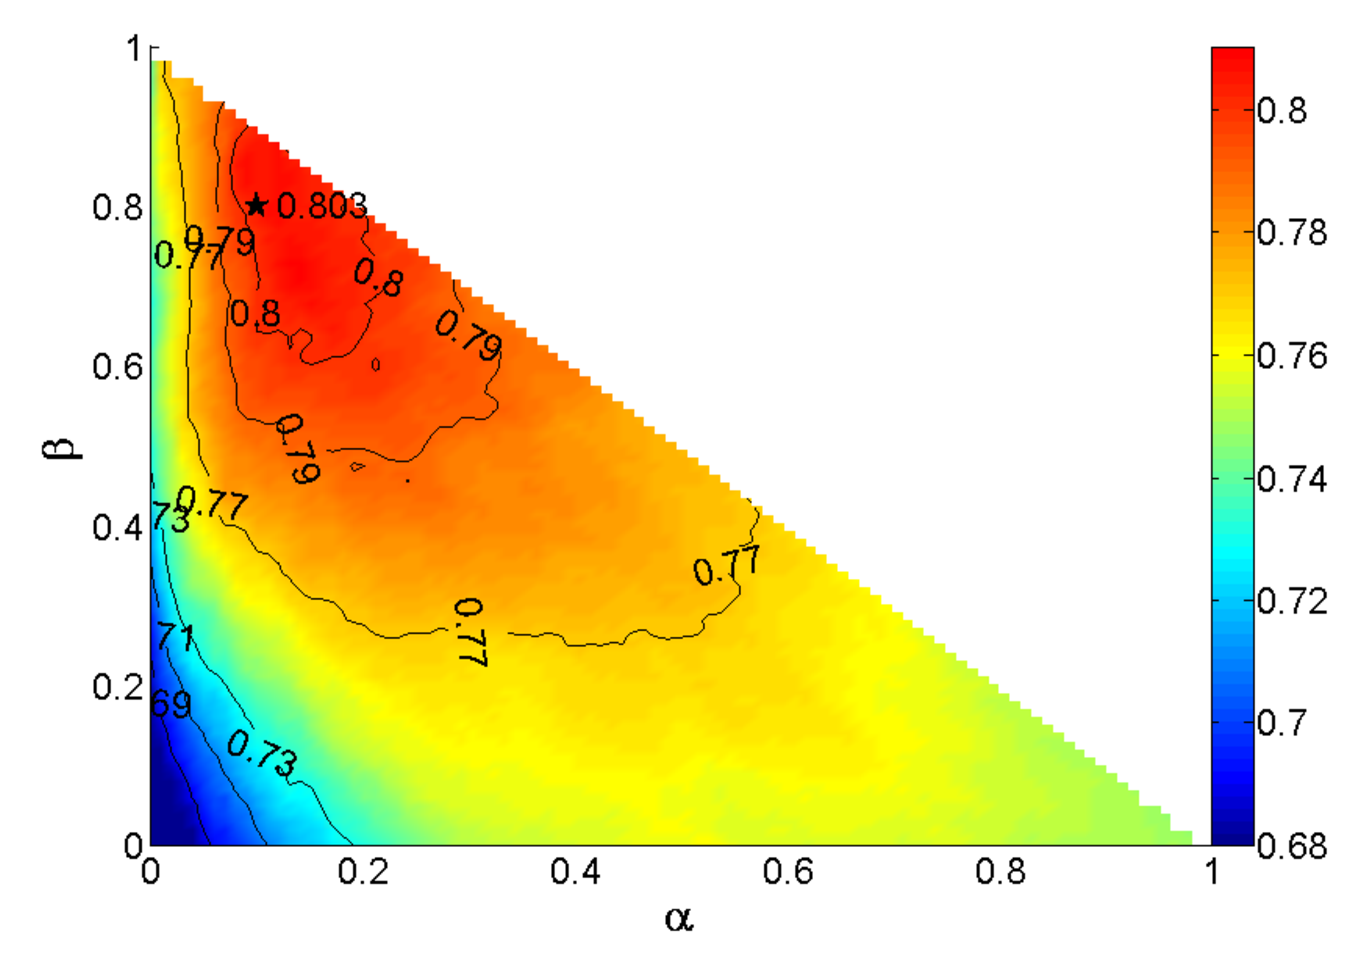
\includegraphics[scale=\graphscaleexpapp]{./exp/AAN-para-recm.eps}}
%\quad\quad
%\hspace{\graphmarginexpapp}
\hfill
\subfigure[{\scriptsize \aminer with \recom}]{\label{exp-aminer-ab-recom}
\includegraphics[scale=\graphscaleexpapp]{./exp/AMiner-para-recm.eps}}
%\quad\quad
%\hspace{\graphmarginexpapp}
\hfill
\subfigure[{\scriptsize \magdata with \recom}]{\label{exp-mag-ab-recom}
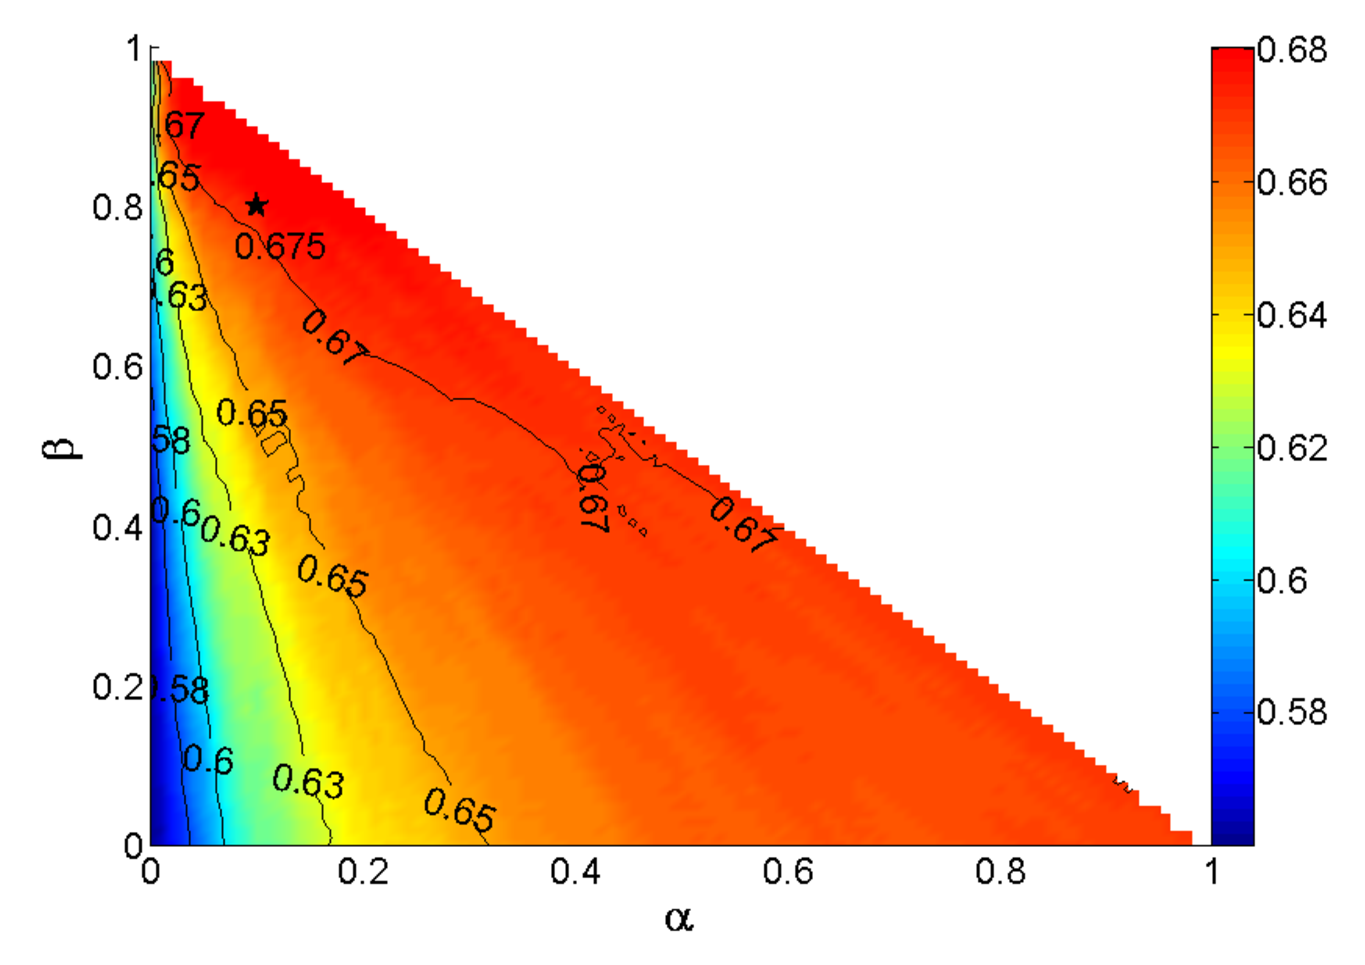
\includegraphics[scale=\graphscaleexpapp]{./exp/MAG-para-recm.eps}}
\\ %%%%%%%%%%%%%%%%%%%%%%%%%%%%%%%%%%%%%%
\vspace{-2ex}
%\hspace{-10ex}
\subfigure[{\scriptsize \aan  with \fcita}]{\label{exp-aan-ab-fcita}
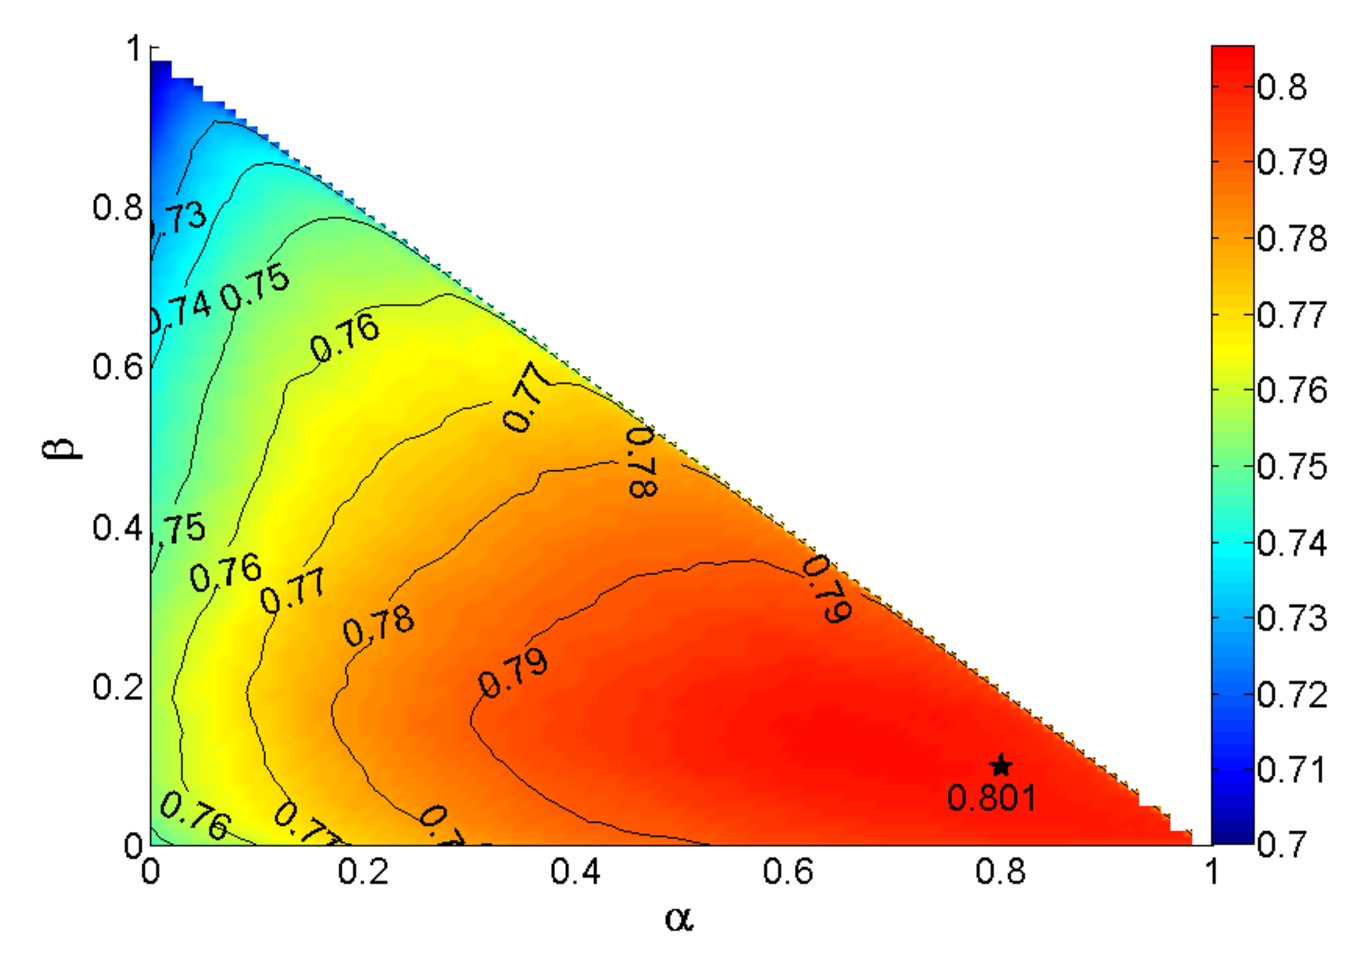
\includegraphics[scale=\graphscaleexpapp]{./exp/AAN-para-fcita.eps}}
%\quad\quad
%\hspace{\graphmarginexpapp}
\hfill
\subfigure[{\scriptsize \aminer with \fcita}]{\label{exp-aminer-ab-fcita}
\includegraphics[scale=\graphscaleexpapp]{./exp/AMiner-para-fcita.eps}}
%\quad\quad
%\hspace{\graphmarginexpapp}
\hfill
\subfigure[{\scriptsize \magdata with \fcita}]{\label{exp-mag-ab-fcita}
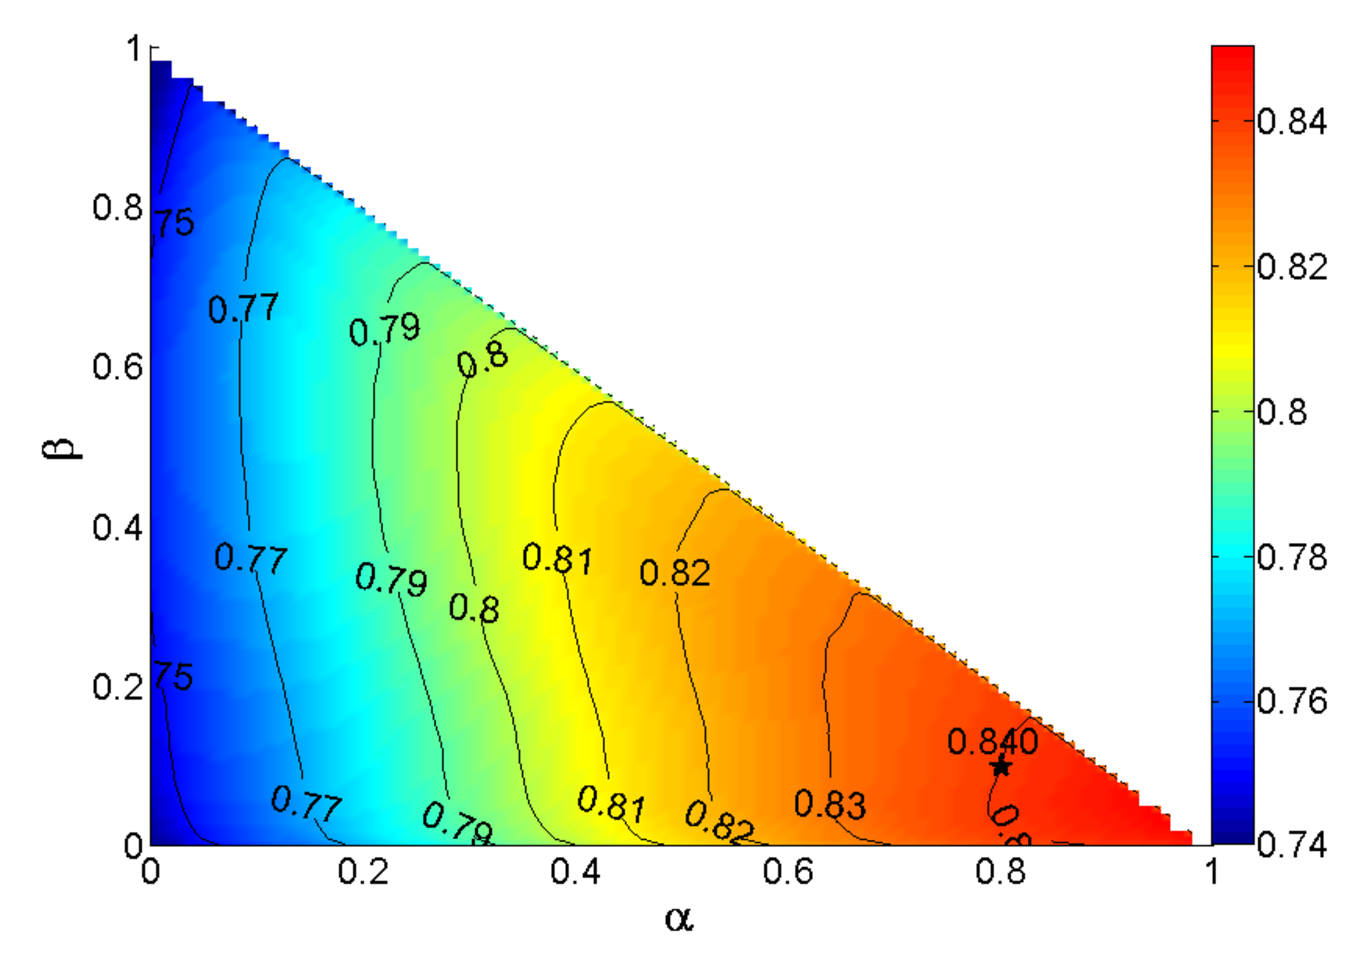
\includegraphics[scale=\graphscaleexpapp]{./exp/MAG-para-fcita.eps}}
\end{center}
\vspace{-2.5ex}
\caption{\small Accuracy tests: varying aggregating parameters $\alpha$ and $\beta$}
\label{exp-ab}
\vspace{-3ex}
\end{figure*}
%%%%%%%%%%%%%%%%%%%%%%%%%%%%%%%%%%%%%%

\stitle{Exp-4: Impacts of parameters}.
%\subsubsection{Exp-4: Impacts of parameters}.
In the last set of tests, we evaluated the impacts of time decaying factor $\sigma$, importance weighting factor $\lambda$, aggregating parameters $\alpha$ and $\beta$, and the TWPageRank. We fixed these parameters as well as $Y_s$ to their default values, used the TWPageRank proposed in this work by default, and tested the \PairAcc with the entire \recom and \fcita (\ie $T_i=+\infty$, $dif=1$).

%We present main results only and more details are available in~\cite{SARank-full}.




\etitle{Exp-4.1}.
%\stitle{Exp-4.1}.
To evaluate the impacts of the time decaying factor $\sigma$, we varied $\sigma$ from -1.6 to -0.4.
%, while fixed $Y_s$ to default values, $T_i=+\infty$, $dif=1$ and $\lambda=0.5$.
The results of \PairAcc are reported in Figs.~\ref{exp-aan-sigma}, \ref{exp-aminer-sigma} and \ref{exp-mag-sigma}.
%with both sets of ground-truth


When varying $\sigma$, the \PairAcc of \ensemblerank is very stable on all datasets using both \recom and \fcita. Indeed, with \recom and \fcita, the \PairAcc only varies (0.42\%, 1.55\%, 0.81\%) and (1.26\%, 0.96\%, 1.16\%) on (\aan, \aminer, \magdata), respectively.
%
%We omitted the detailed results of running time due to space constraint.
The running time varies (11.3\%, 8.6\%) on average only on (\aminer, \magdata), respectively.
%(0.18, 33.6) seconds, \ie

%Both of these show the robustness of \ensemblerank to the time decaying factor $\sigma$.

%As we can see from the figure, our method \ensemblerank is almost stable with the reduction of $\sigma$, since there is only a small fluctuation and the accuracy of our methods is always higher than the best baseline result in all datasets regardless of the change of $\sigma$. This means \ensemblerank is insensitive with $\sigma$.


%%%%%%%%%%%%%%%%%%%%%%%%%%%%%%%%%%%%%%%%%%%%%%%%%%
\begin{table}[tb!]
%\vspace{-2ex}
\begin{center}
\caption{\small Accuracy tests using different components with \recom (rows 2--4) and \fcita (rows 5--7).}
\label{tab-recom}
\begin{small}
\vspace{-.5ex}
\begin{tabular}{|c| c |c | c|}
\hline
{\bf Datasets} & {\bf C}\hspace{5ex}{\bf V}\hspace{5ex}{\bf A} & {\bf CV}\hspace{3ex}{\bf CA}\hspace{3ex}{\bf VA} & {\bf CVA} \\
\hline \hline
% \recom
\aan & 0.752 \ 0.616 \ 0.649 & 0.809 \ 0.764 \ 0.747 & {\bf 0.810} \\
\aminer & 0.735 \  0.581 \  0.640 & 0.784 \ 0.749 \ 0.729 & {\bf 0.785} \\
\magdata & 0.635 \ 0.534 \ 0.553 & 0.697 \ 0.673 \  0.648 & {\bf 0.698} \\ \hline
% \ficta
\aan & 0.785 \ 0.557 \ 0.761 & 0.849 \ 0.866 \ 0.771 & {\bf 0.870} \\
\aminer & 0.713 \  0.603 \  0.725 & 0.843 \ 0.847 \ 0.740 & {\bf 0.856} \\
\magdata & 0.736 \ 0.628 \ 0.718 & 0.848 \ 0.857 \ 0.751 & {\bf 0.874} \\
\hline
\end{tabular}
\end{small}
\end{center}
\vspace{-6ex}
\end{table}
%%%%%%%%%%%%%%%%%%%


\etitle{Exp-4.2}.
%\stitle{Exp-4.2}.
To evaluate the impacts of importance weighting factor $\lambda$, we varied $\lambda$ from 0 to 1.
%while fixed $Y_s$ to default values, $T_i=+\infty$, $dif=1$ and $\sigma=-1.0$.
The results of \PairAcc are reported in Figs.~\ref{exp-aan-lambda}, \ref{exp-aminer-lambda} and \ref{exp-mag-lambda}. Note that parameter $\lambda$ has no impacts on efficiency.
%with both sets of ground-truth

When varying $\lambda$, the \PairAcc of \ensemblerank first increases and then decreases on all datasets with both \fcita and \recom, except on \aminer with \recom.
%\marked{The value of $\lambda$ for \ensemblerank to achieve the best effectiveness is (0.6, 0, 0.2) and (0.6, 0.4, 0.1) on (\aan, \aminer, \magdata) with \recom and \fcita, respectively.}
This result indicates that combining prestige and popularity generally produces more robust results than using either of prestige and popularity.
Indeed, with \recom and \fcita, the \PairAcc of combining prestige and popularity is (10.2\%, 10.7\%, 5.5\%) and (8.0\%, 8.7\%, 9.0\%) higher than using prestige alone, and is (1.2\%, -0.1\%, 1.0\%) and (1.0\%, 1.0\%, 0.3\%) higher than using popularity alone on (\aan, \aminer, \magdata), respectively.


%The selection of $\lambda$ is influenced by ground-truth, such that the best $\lambda$ falls into $[xx,xx]$ and $[yy,yy]$ on \fcita and \recom, respectively. Moreover, equally weighting, \ie $\lambda=0.5$, is a good default setting when no query information is available in advance.
%Indeed, the best obtained \PairAcc using (\fcita, \recom) is only (0.10\%, 0.38\%), (0.04\%, 2.59\%) and (0.06\%, 0.91\%)  higher than the \PairAcc of equally weighting on \aan, \aminer and \magdata, respectively.





\etitle{Exp-4.3}.
To evaluate the impacts of aggregating parameters $\alpha$ and $\beta$, we varied $\alpha$ and $\beta$ at the granularity of 0.01. Again, parameters $\alpha$ and $\beta$ have few impacts on efficiency. The results are reported in Fig.~\ref{exp-ab}, where the parameters selected earlier and their corresponding \PairAcc are marked with $*$.

When varying $\alpha$ and $\beta$, the \PairAcc of \ensemblerank changes gently, as shown in Fig.~\ref{exp-ab}.
The optimal \PairAcc is obtained within a single region, rather than a complex collection of optimal regions.
%
Moreover, the \PairAcc keeps at a high level within a certain ($\alpha$, $\beta$) combination space around the optimal region, as shown in Fig.~\ref{exp-ab}.
%For instance, consider a square of length 0.3, which covers 8.5\% of the parameter combination space. The fraction of parameters such that the \PairAcc is no worse than 1\% of the corresponding \PairAcc with marker $*$ is (73\%, 94\%) on \aan, (96\%, 87\%) on \aminer and (83\%, 95\%) on \magdata, using (\recom, \fcita), respectively.
%
Further, the optimal parameters on the same sets of ground-truth are very similar for (\aan, \aminer and \magdata), indicating that the setting of $\alpha$ and $\beta$ can be easily transferred across different datasets.
To conclude, \ensemblerank is very robust to parameters $\alpha$ and $\beta$, and it is quite flexible for choosing proper values of parameters $\alpha$ and $\beta$.

Moreover, this enables to verify the effectiveness of importance assembling from different components, whose results are reported in Table~IV, in which letters C, V and A stand for citation, venue and author components, respectively.
The ranking based on all components consistently performs the best, using both \recom and \fcita, which justifies the use of importance assembling for ranking scholarly articles.
%which, using \recom and \fcita, improves the \PairAcc over using components (C, V, A, CV, CA, VA) by (5.77\%, 19.4\%, 16.1\%, 0.09\%, 4.59\%, 6.28\%) and (9.54\%, 23.7\%, 5.90\%, 2.50\%, 0.71\%, 4.79\%) on \aan, (6.94\%, 23.7\%, 14.4\%, 0.21\%, 1.56\%, 7.67\%) and (17.68\%, 12.4\%, 9.61\%, 0.33\%, 1.88\%, 6.34\%) on \aminer, and (6.29\%, 16.38\%, 14.45\%, 0.05\%, 2.43\%, 5.02\%) and (11.43\%, 19.2\%, 11.2\%, 1.44\%, 0.77\%, 9.62\%) on \magdata, respectively.


\eat{
\etitle{Exp-4.3}.
%\stitle{Exp-4.3}.
To evaluate the impacts of aggregating parameters $\alpha$ and $\beta$, we varied $\alpha$ and $\beta$ at the granularity of 0.01.
%while fixed $Y_s$ to default values, $T_i=+\infty$, $dif=1$, $\sigma=-1.0$ and $\lambda=0.5$.
Again, parameters $\alpha$ and $\beta$ have few impacts on efficiency. Due to space limitations, we only present the main results and more details are available at~\cite{SARank-full}.

Indeed, \ensemblerank is very robust to parameters $\alpha$ and $\beta$.
(a) When varying $\alpha$ and $\beta$, the \PairAcc of \ensemblerank changes gently. (b) \PairAcc also keeps at a high level within a certain ($\alpha$, $\beta$)  combination space. Finally, (c) the optimal parameters on the same set of ground-truth are very similar for \aan, \aminer and \magdata. That is, it is quite flexible for choosing proper values
of  parameters $\alpha$ and $\beta$.
} %%%%%%%% brief version of Exp-4.3

%%%%%%%%%%%%%%%%%%%%%%%%%%%%%%%%%%%%%%
\begin{figure*}[tb!]
%\vspace{1ex}
\addtolength{\subfigcapskip}{-1ex}
\begin{center}
\subfigure[{\scriptsize \aan with \recom}]{\label{exp-aan-recom-drank}
\includegraphics[scale=0.35]{./exp/AAN_TWPageRank_recom.eps}}
\hfill
%\hspace{\graphmarginexpapp}
\subfigure[{\scriptsize \aminer with \recom}]{\label{exp-aminer-recom-drank}
\includegraphics[scale=0.35]{./exp/AMiner_TWPageRank_recom.eps}}
\hfill
%\hspace{\graphmarginexpapp}
\subfigure[{\scriptsize \magdata with \recom}]{\label{exp-mag-recom-drank}
\includegraphics[scale=0.35]{./exp/MAG_TWPageRank_recom.eps}}
\\%%%%%%%%%%%%%%%%%%%%%%%%%%%%%%%%%%%%%%%%%%%
\vspace{-1.5ex}
\subfigure[{\scriptsize \aan with \fcita}]{\label{exp-aan-fcita-drank}
\includegraphics[scale=0.35]{./exp/AAN_TWPageRank_fcita.eps}}
\hfill
%\hspace{\graphmarginexpapp}
\subfigure[{\scriptsize \aminer with \fcita}]{\label{exp-aminer-fcita-drank}
\includegraphics[scale=0.35]{./exp/AMiner_TWPageRank_fcita.eps}}
\hfill
%\hspace{\graphmarginexpapp}
\subfigure[{\scriptsize \magdata with \fcita}]{\label{exp-mag-fcita-drank}
\includegraphics[scale=0.35]{./exp/MAG_TWPageRank_fcita.eps}}
\end{center}
\vspace{-2.5ex}
\caption{\small Impacts of the TWPageRank on accuracy: varying importance weighting
factor $\lambda$}
\label{exp-drank}
\vspace{-3ex}
\end{figure*}
%%%%%%%%%%%%%%%%%%%%%%%%%%%%%%%%%%

\newcommand{\drank}{\kw{DRank}}


\etitle{Exp-4.4}.
\marked{To evaluate the impacts of the proposed TWPageRank, we compared our approach \ensemblerank with an algorithm alternative (referred to as \drank) the same to \ensemblerank except exploiting exponentially decayed impact weights, \ie $w(u,v)=e^{\sigma(T_u-T_v)}$ in Eq.~(\ref{eq-infl-weights}).
%The two algorithms produce the same popularity while different prestige.
To better understand the impacts, we varied the importance weighting factor $\lambda$ from 0.1 to 1. Note that the ranking results are the same when $\lambda=0$ due to the same popularity computation. The results are reported in Fig.~\ref{exp-drank}, where the numbers represent the improvement of \PairAcc by \ensemblerank over the one by \drank.}

\marked{
When varying $\lambda$, the \PairAcc of \ensemblerank is better than the one of \drank in most cases, which shows the superiority of the TWPageRank than exploiting exponentially decayed weights.
The difference of \PairAcc by the two algorithms is higher with \recom than with \fcita, since the two algorithms are using citation information to predict past and future citations with \fcita.
Moreover, algorithm \ensemblerank is consistently better than \drank when $0.5 \le \lambda \le 0.9$.
%, which, with \recom and \fcita, improves the \PairAcc by (2.88\%, 3.91\%, 3.90\%) and (0.55\%, 0.50\%, 0.22\%) on (\aan, \aminer, \magdata) on average, respectively.
The improvement decreases with the decrease of $\lambda$ as the popularity dominates the ranking with small $\lambda$, and in some cases, \drank outperforms \ensemblerank. %as the prestige and popularity orders of article pairs are more diverse for \drank than \ensemblerank.
Overall, with \recom and \fcita, \ensemblerank improves the \PairAcc over \drank by (1.78\%, 3.07\%, 3.20\%) and (0.29\%, 0.48\%, 0.11\%) on (\aan, \aminer, \magdata) on average, respectively.
}

\marked{
The TWPageRank has little impacts on efficiency, and the running time of the two algorithms only varies (6.34\%, 4.83\%) on (\aminer, \magdata) on average, respectively.}

\eat{
With the increment of $\lambda$, \ensemblerank has more promotion than DRank and the \PairAcc of DRank is better than \ensemblerank with small $\lambda$, possibly due to the addition of popularity will correct the mistaken pairs better on DRank, although \ensemblerank rank more pairs correctly.
In addition, the change of \PairAcc with \recom is higher than the one with \fcita, possibly due to the article pairs in \fcita are of the same years.
Moreover, the \PairAcc of \ensemblerank is better than its counterparts from $\lambda=0.5$ to $\lambda=1$, except on \aminer with \fcita. Recall that in Fig.~\ref{exp-aminer-lambda} using popularity alone gives the best results on \aminer, indicating that the prestige computed by TWPageRank is less accurate on \aminer than on the other two datasets.
%
Indeed, with \recom and \fcita, the \PairAcc of \ensemblerank is (2.20\%, 6.63\%, 5.68\%) and (0.25\%, 0.05\%, 0.05\%) higher than DRank on (\aan, \aminer, \magdata), respectively, when using prestige alone, and is (1.73\%, 2.97\%, 2.92\%) and (0.22\%, -0.08\%, 0.17\%) higher when combining prestige and popularity, respectively, on average.
%
Finally, the TWPageRank has little impacts on efficiency, and the running time of \ensemblerank and its counterparts only changes (6.34\%, 4.83\%) on (\aminer, \magdata) on average, respectively.
}

\stitle{Summary}.
From these tests we find the followings.


\sstab(1) Our model \ensemblerank is effective for ranking scholarly articles, which is consistently better than competitive methods in all tests. With \recom and \fcita, \ensemblerank improves \PairAcc over (\pagerank, \futurerank, \hhgrank) by
(13.5\%, 6.8\%, 4.8\%) and (12.0\%, 3.0\%, 3.2\%) on \aan,
(12.7\%, 5.0\%, 4.9\%) and (14.0\%, 6.5\%, 4.6\%) on \aminer, and
(6.5\%, 2.5\%, 2.2\%) and (13.4\%, 6.0\%, 2.4\%) on \magdata, on average, respectively.
%, and it has a great advantage in evaluating the importance in a long term. Furthermore, it is more accurate evaluating articles which have just published and is in lack of citations, since it uses both venue network and author information besides of citation network. Indeed, it improves the accuracy by $(7.9\%, 3.2\%, 2.3\%)$ and $(14.4\%, 5.0\%, 3.8\%)$ over \pagerank, \futurerank and \hhgrank on average of three datasets with recommendation based ground truth and future citation ground truth, respectively.


\sstab(2) Our batch algorithm \batensemble and incremental algorithm \incensemble are also efficient.
%
Our incremental algorithm \incensemble is on average (1.7, 3.1, 2.8, 117) and (2.0, 3.0, 4.4, 245) times faster than (\batensemble, \powensemble, \futurerank, \hhgrank)  on the large \aminer and \magdata, respectively.

%The batch algorithm \batensemble is on average (1.3, 2.5, 348) times faster than (\powensemble, \futurerank, \hhgrank)  on the largest \magdata, respectively.

%\noindent (3) Our incremental algorithms are much faster than their batch counterparts in practice, even their time complexity is very close. Indeed, algorithms \inctwprdag, \inctwprscc and \incensemble further improve the efficiency of (\twprdag, \twprscc, \batensemble) by (23\%, 38\%, 22\%) on average, respectively.


\sstab(3) Our ranking model \ensemblerank introduces the time decaying factor $\sigma$, importance weighting factor $\lambda$ and aggregating parameters $\alpha$ and $\beta$ for the sake of practicability and flexibility in real-life applications, and, from our tests, \ensemblerank is very robust to these parameters. Moreover, the proposed TWPageRank is generally more effective than directly using exponentially decayed impact weights.




\stitle{Related work}. We summarize related work as follows.
%
%Scholarly article ranking

Scholarly article ranking has shifted from citation count analysis~\cite{Garfield471,Hirsch15112005} to graph analysis~\cite{ChenXMR07,Zhou07-CoRank,Jiang12-MRank,Liang16AAAI,Li08TSRanking,Wang13AAAI,WalkerXKM07,sayyadi09,
Wang16TIST,Ng11KDD}.
Based on the information used, these methods are divided into four categories: (a) using the citation information only~\cite{Garfield471,Hirsch15112005,ChenXMR07,Ng11KDD}, (b) using the citation and temporal information~\cite{Li08TSRanking,WalkerXKM07}, (c) using the citation information and other heterogeneous information, \eg authors and venues of articles~\cite{Zhou07-CoRank,Jiang12-MRank,Liang16AAAI}, and (d) combining the citation, temporal and other heterogeneous information~\cite{sayyadi09,Wang16TIST,Wang13AAAI}.
Our work belongs to the last category aiming at fully employing information available for scholarly article ranking.


%\stitle{PageRank\&weighted PageRank algorithms}.

%PageRank \cite{Brin98:PageRank} and its extensions have been extensively used for citation analyses \cite{Waltman2014}. While PageRank equally propagates scores along outlinks, Weighted PageRank \cite{Xing04:WPR} extends PageRank by distributing scores based on the popularity of pages. Different from previous work, the Time-Weighted PageRank proposed in this work discriminately propagates scores in terms of citation statistics.

PageRank \cite{Brin98:PageRank} and its extensions have been extensively used for citation analyses \cite{Waltman2014}. While PageRank equally propagates scores along outlinks, Weighted PageRank extends PageRank by distributing scores based on certain criteria such as popularity of pages~\cite{Xing04:WPR} or authority of authors~\cite{Ding11}. Different from previous work, the Time-Weighted PageRank proposed in this work discriminately propagates scores in terms of citation statistics.






%\stitle{Dynamic algorithms}.

Dynamic algorithms have proven useful for various tasks by avoiding computing from scratch~\cite{RamalingamR93}.
% and only recomputing those affected by updates
%Dynamic algorithms have proven useful for graph analysis tasks, \eg incremental graph pattern matching~\cite{FanWW13} and  incremental simrank computation~\cite{YuLZ14}.
To our knowledge, little concern has been paid to dynamic scholarly article ranking except that~\cite{GhoshKHLL11} uses PageRank in dynamic citation networks. However, its solution is based on a strong and impractical assumption that there are no citations between articles in the same years.
Further, although there exist several studies on incremental PageRank computation~\cite{DesikanPSK05,AbiteboulPC03,WuR09} and on incremental PageRank approximation \cite{BahmaniCG10,BahmaniKMU12}, they are not designed for scholarly article ranking.
%
Different from previous work, we study scholarly article ranking in a dynamic environment in terms of
the citation characteristics of scholarly articles, which has never been exploited before.

%Our approach only makes the assumption that there are no mutual references within the citation network, which, we admit, violates xx\% of total citations on \magdata, and is significantly different (yy\% on \magdata) from~\cite{GhoshKHLL11}.  - move to Section 3

Ensemble methods use multiple learners to obtain better performance than could be obtained from a constituent learner alone~\cite{zhihua-book}.
%In this work, we leverage ensembles to produce better and robust results for scholarly article ranking~\cite{zhihua-book,wsdmcup,DuanAMHH16}.
In this work, we leverage  importance assembling  to produce better and robust results for scholarly article ranking~\cite{zhihua-book,wsdmcup,DuanAMHH16}.

\vspace{-1ex}
%%%%%%%%%%%%%%%%%%%%%%%%%%%%%%%%%%%%%%%%%%%%%%%%%%%%%%%%%%%%%%%%%%%%%%%%%%%%%%
\section{Conclusions}
%%%%%%%%%%%%%%%%%%%%%%%%%%%%%%%%%%%%%%%%%%%%%%%%%%%%%%%%%%%%%%%%%%%%%%%%%%%%%%

We have evaluated the state-of-the-art \lsa algorithms for trajectory compression, including \emph{both the optimal and the sub-optimal methods that use either \ped or \sed}. 
Using a variety of real trajectory datasets, we evaluated the performance of each technique.% in terms of its processing time, compression ratio and average error.
Our experimental results show that 
(1) the output sizes of algorithms using \sed are approximate $2$ times of using \ped, 
(2) the output sizes of sub-optimal algorithms are $130\%$--$160\%$ of the optimal algorithms, and 
(3) the one-pass algorithms \siped and \operb and \cised are tens of times faster than the batch algorithms and \textcolor{red}{$xxx$} times faster than online algorithms, while they still have comparable compression ratios with batch algorithms. Hence, they are more suitable for resource constraint mobile devices.


% use section* for acknowledgment
% The Computer Society usually uses the plural form
\section*{Acknowledgments}
This work is supported in part by NSFC (U1636210) and 973 program ({2014CB340300}).
\textcolor{blue}{We would like to thank Yanchen Hou for running the experiments, and all the referees for their valuable comments.}

\section*{{Appendix:  Proofs}}





\stitle{Proof of Theorem~\ref{theo-ldrh-cised}}:
\todo{1. $\vv{v}$ in 3D space; 2...}

If $|P_{s+i}P'_{s+i}|\le \epsilon/2$ for each $i \in [1,k]$, then $\vv{v}$ must live in the common intersection of half-$\epsilon$ cones $\bigsqcap_{i=1}^{k}$\cone{(P_s, P_{s+i}, \epsilon/2)}, where $P'_{s+i}$ is the synchronized point of $P_{s+i}$ \wrt velocity $\vv{v}$.
\eop

\stitle{Proof of Theorem~\ref{theo-full-cone}}:
\todo.
\eop

\stitle{Proof of Theorem~\ref{theo-cone-vs}}:
\todo.
\eop

\stitle{Proof of Theorem~\ref{theo-half-sector}}:
Trajectory tracking is the combination of trajectory simplification and position tracking.
%
(1) Trajectory simplification: It can be simplified in strip-like areas as shown in Section \ref{sec:sector-in-simp};
%
(2) Position tracking: If it can be represented by a line segment by the intersection of sectors, then there is sure a $\vv{v}$ living in the common intersection of sectors, \eg $\vv{v}$ on $P_sP_{s+i}$, such that it is applicable to track the position in strip areas.
%
Combine (1) and (2), we have the conclusion.
\eop

\stitle{Proof of Theorem~\ref{theo-full-sector}}:
\todo.
\eop

\stitle{Proof of Theorem~\ref{theo-sector-vs}}:
\todo.
\eop

\stitle{Proof of Theorem~\ref{theo-binary}}:
\todo.
1. traj simplification by cones and sectors.
2. position tracking: one velocity, from the intersection of cones.
\eop



\balance
%\begin{footnotesize}
\bibliographystyle{abbrv}
\bibliography{sec-ref}
%\end{footnotesize}





% that's all folks
\end{document}
